\documentclass[a4paper,10pt]{article}
\usepackage[utf8]{inputenc}

% ----  Useful packages % ---- 
\usepackage{amsmath}
\usepackage{graphicx}
\usepackage{amsfonts}
\usepackage{amsthm}
\usepackage{amssymb}
\usepackage{makecell}
\usepackage{array}
\usepackage{booktabs}
\usepackage{multirow}
\usepackage{subfigure}
% ----  Useful packages % ---- 

\usepackage{wrapfig}
\usepackage{caption}
\usepackage{subcaption}
\usepackage{hyperref}
\hypersetup{
    colorlinks,
    citecolor=black,
    filecolor=black,
    linkcolor=black,
    urlcolor=black
}

\graphicspath{ {./images/} }

% ---- Set page size and margins replace ------
\usepackage[letterpaper,top=2cm,bottom=2cm,left=3cm,right=3cm,marginparwidth=1.75cm]{geometry}
% ---- Set page size and margins replace ------

% ------- NOTA ------
\theoremstyle{remark}
\newtheorem{note}{Note}[subsubsection]
% ------- NOTA ------

% ------- OSSERVAZIONE ------
\theoremstyle{definition}
\newtheorem{observation}{Observation}[subsection]
% ------- OSSERVAZIONE ------

% ------- DEFINIZIONE ------
\theoremstyle{plain}
\newtheorem{definition}{Definition}[subsection]
% ------- DEFINIZIONE ------

% ------- ESEMPIO ------
\theoremstyle{definition}
\newtheorem{example}{Example}[subsection]
% ------- ESEMPIO ------

% ------- DIMOSTRAZIONE ------
\theoremstyle{definition}
\newtheorem{question}{Question}[subsection]
% ------- DIMOSTRAZIONE ------

% ------- TEOREMA ------
\theoremstyle{definition}
\newtheorem{theorem}{Theorem}[subsection]
% ------- TEOREMA ------

% ------- COROLLARIO ------
\theoremstyle{plain}
\newtheorem{corollaries}{Corollario}[theorem]
% ------- COROLLARIO ------

% ------- PROPOSIZIONE ------
\theoremstyle{plain}
\newtheorem{proposition}{Proposizione}[subsection]
% ------- PROPOSIZIONE ------

% ---- Footer and header ---- 
\usepackage{fancyhdr}
\pagestyle{fancy}
\fancyhf{}
\fancyhead[LE,RO]{A.A 2024-2025}
\fancyhead[RE,LO]{Telematics}
\fancyfoot[RE,LO]{\rightmark}
\fancyfoot[LE,RO]{\thepage}

\renewcommand{\headrulewidth}{.5pt}
\renewcommand{\footrulewidth}{.5pt}
% ---- Footer and header ---- 

% ----  Language setting ---- 
\usepackage[italian, english]{babel}
% ----  Language setting ---- 

\usepackage{listings}
\usepackage{color}

\definecolor{dkgreen}{rgb}{0,0.6,0}
\definecolor{gray}{rgb}{0.5,0.5,0.5}
\definecolor{mauve}{rgb}{0.58,0,0.82}

\lstset{frame=tb,
  language=C,
  aboveskip=3mm,
  belowskip=3mm,
  showstringspaces=false,
  columns=flexible,
  basicstyle={\small\ttfamily},
  numbers=none,
  numberstyle=\tiny\color{gray},
  keywordstyle=\color{blue},
  commentstyle=\color{dkgreen},
  stringstyle=\color{mauve},
  breaklines=true,
  breakatwhitespace=true,
  tabsize=3
}

\setcounter{tocdepth}{4}

\title{\textbf{Telematics}}
\author{Autor: Ghirardini Filippo}
\date{Winter Semester 2024-2025}

\begin{document}
\begin{titlepage} %crea l'enviroment
	\begin{figure}[t] %inserisce le figure
		\centering
\includegraphics[width=0.98\textwidth]{marchio_unipi_pant541.png}
	\end{figure}
	\vspace{20mm}
	
	\begin{Large}
		\begin{center}
			\textbf{Dipartimento di Informatica\\ Corso di Laurea Triennale in Informatica\\}
			\vspace{20mm}
			{\LARGE{Corso a Libera Scelta - 6 CFU}}\\
			\vspace{10mm}
			{\huge{\bf Computer Graphics}}\\
		\end{center}
	\end{Large}
	
	
	\vspace{36mm}
	%minipage divide la pagina in due sezioni settabili
	\begin{minipage}[t]{0.47\textwidth}
		{\large{\bf Professore:}\\ \large{Prof. }}
	\end{minipage}
	\hfill
	\begin{minipage}[t]{0.47\textwidth}\raggedleft
		{\large{\bf Autore:}\\ \large{Filippo Ghirardini}}
	\end{minipage}
	
	\vspace{25mm}
	
	\hrulefill
	
	\vspace{5mm}
	
	\centering{\large{\bf Anno Accademico 2023/2024 }}
	
\end{titlepage}

\tableofcontents
\newpage
\maketitle
\begin{center}
    \vspace{-20pt}
    \rule{11cm}{.1pt} 
\end{center}
\newpage
\section{Basics}
\subsection{Network composition}
A network consists of three elements:
\begin{itemize}
	\item \textbf{End systems}: can vary in size and usage
	\item \textbf{Intermediate systems}: these (e.g. routers) are the components that allow the network to work.
	\item \textbf{Links}: they connect the end systems and can be \textit{optical}, \textit{copper} or \textit{wireless}. Even if wireless is becoming more and more important, cables are still fundamental (undersea cables, underground cables).
\end{itemize}

\begin{question}[Why fiber optic?]
	Because this medium has not reached it's maximum and still has a huge potential of \textbf{bandwidth}. Also, while copper cable start acting as an \textbf{antenna} (and a receiver), disturbing near copper cable, fiber optic doesn't have this problem. Furthermore, copper cables need amplifiers which increase \textbf{latency}.
\end{question}

\begin{question}[Why copper?]
	It's \textbf{cheaper} and \textbf{easier} to handle.
\end{question}

\begin{question}[Why cables over wireless?]
	Because of \textbf{stability} and \textbf{latency}. Usually the problem is tampered by buffers but obviously it doesn't work with interactive applications.
\end{question}

\begin{question}[What are threats to cable?]
	
\end{question}

\subsection{Communication principles}
There are two basics principles:
\begin{itemize}
	\item \textbf{Synchronous}: joint action of sender and receiver. Requires \textbf{waiting} until all parties are ready (e.g. phone calls)
	\item \textbf{Asynchronous}: sender and receiver operate decoupled (e.g. SMS, email). Requires \textbf{buffering}.
\end{itemize}

\begin{note}
	There is also \textbf{isochronous}, which means the messages are sent every predetermined amount of time.
\end{note}

\subsubsection{Direction}
Communication channels may allow traffic flow in different directions:
\begin{itemize}
	\item \textbf{Simple duplex}: one direction
	\item \textbf{Half-duplex}: both directions in different moments
	\item \textbf{Full-duplex}: both directions at the same time
\end{itemize}
\subsubsection{Distribution}
The communication distribution can happen in different ways:
\begin{itemize}
	\item \textbf{Unicast}: one to one
	\item \textbf{Broadcast}: one to all
	\item \textbf{Multicast}: one to a subset
	\item \textbf{Anycast}: one to the nearest, e.g. when requesting to a redundant database you don't care which one responds
	\item \textbf{Concast}: many to one, e.g. we collect sensor data and send it to one
	\item \textbf{Geocast}: one to a certain region
\end{itemize}
\begin{note}
	Even if multicast would be easier and cheaper, companies usually go for unicast because they want to know who the clients are.
\end{note}

\begin{note}
	Broadcast guarantees anonymity while multicast does not.
\end{note}

\subsubsection{Topologies}
The main topologies are:
\begin{itemize}
	\item \textbf{Full mesh}: too expensive
	\item \textbf{Chain}: in cars and trains
	\item \textbf{Star}: ideal for switches
	\item \textbf{Partial mesh}: the best compromise
	\item \textbf{Tree}: not ideal for big networks since if you cut a side, you lose contact
\end{itemize}

\subsection{Sharing}
\subsubsection{Cons}
Sharing may create a lot of problems, like \textbf{bottlenecks}: links and intermediate nodes are shared between end systems. One solution may be to \textit{reroute} or to start \textit{dropping packets} (e.g. when streaming the resolution lowers down).
\subsubsection{Pros}
At the same time, sharing means more efficient (less expensive) mechanism to \textbf{exchange data} between different components of distributed systems and \textbf{minimize blocking} due to multiplexing.

\subsubsection{How?}
There are two possible ways of sharing:
\begin{itemize}
	\item \textbf{Reservation}: you reserve in advance the resource so that it is guaranteed, e.g. remote surgery. When the peak demand and the flow duration varies, there are two options:
	\begin{enumerate}
		\item \textit{First Come First Served}
		\item Everyone gets $10Mbps$
	\end{enumerate}
	It is implemented with \textbf{circuit-switching}: establishes dynamically a dedicated communication channel. It has predictable performance and a simple and fast switching but it's inefficient for bursty traffic, complex to setup and not easily adaptive to failures.
	
	\item \textbf{On-demand}: when there is a resource available you take it (variable \textit{delay}, \textbf{jitter}), e.g. email. It is implemented with \textbf{packet-switching}: splitting the resource in packets and multiplex them. Much more flexible but requires buffers, packets overhead and has unpredictable performances.
\end{itemize}

\begin{observation}
	It all depends on the application. Each flow has a \textbf{peak rate} and an \textbf{average rate}.To decide if \textit{reservation} works well for a specific case, we must look at the ratio $\frac{P}{A}$. If it's small then it works well, otherwise it's wasting resources.
\end{observation}
\newpage
\section{DNS}
\subsection{Introduction}
Names provide a level of abstraction from the IP address: for humans it's easier to remember. It also provides \textbf{load balancing} and easy \textbf{aliasing}.\\
The decision for DNS adding is handled by two organizations:
\begin{itemize}
	\item \textbf{IETF}: how entries are entered and read from the phone book
	\item \textbf{ICANN}: how to decide \textit{what} names should be entered in the phone book
\end{itemize}
To use naming you need two things:
\begin{itemize}
	\item \textbf{Unique} names
	\item \textbf{Resolution} of names to locator (IP address) or other services
\end{itemize}

\subsubsection{Scaling}
To allow scaling, DNS uses \textbf{delegation} and \textbf{caching}. In particular for delegation, DNS adopts three intertwined \textbf{hierarchies}:
\begin{itemize}
	\item \textbf{Name space}: hierarchy of names
	\item \textbf{Management}: hierarchy of authorities over names. Who owns which name part.
	\item \textbf{Infrastructure}: hierarchy of DNS server. Where is the mapping stored.
\end{itemize}

\subsection{Namespace}
DNS namespace is implemented as a tree structure: each node has a \textbf{label} which identifies it relatively to its parent node. Each node is \textbf{root} of a sub-tree (if it's not a leaf). In particular direct children of the root are called \textbf{Top Level Domains}. Each subtree represents a \textbf{domain} and each domain can be divided in \textbf{sub-domains}.
\begin{center}
	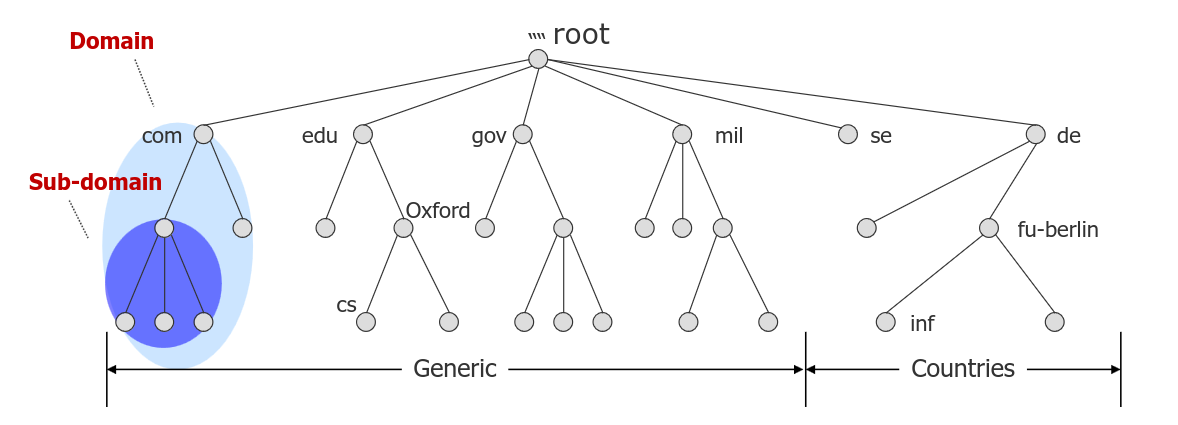
\includegraphics[scale=0.3]{dns_hier.png}
\end{center}
There is a limited number of TLDs: originally it was $7$ plus one for each country. Now there are many more, even in non Latin alphabets.
\subsubsection{Leafs}
The name of a domain consists of a sequence of labels beginning with the root of the domain and going up to the root of the whole tree. Each label is separated by ".".\\
In the leaf nodes the IP addresses are associated with the names.\\
Furthermore, there could be \textbf{Domain Name Aliases}: pointers of one domain to another (Canonical Domain Name).

\subsubsection{DNS Database}
There are a few rules for the database:
\begin{itemize}
	\item The \textbf{depth} of the tree is limited to $127$
	\item Each label can have up to $63$ characters
	\item The whole domain name has a maximum of $255$ characters (even if the average is $10$)
	\item A label of length $0$ is reserved for the root
\end{itemize}
The full address to a host is the \textbf{Fully Qualified Domain Name}, which includes the leaf, each node and the root. The \textbf{Relative Domain Name} instead, is an incomplete domain name.

\subsection{Management}
The management of domain names also follows a hierarchy structure: \textbf{ICANN} manages the root domain and delegates someone (\textbf{DENIC} for Germany) to handle the \textit{de} domain. They then delegate FUB to handle the \textit{fu} domain. And so on.\\
This solution ensures that the names are unique.

\subsection{Name servers and zones}
\subsubsection{Domains}
Domains are administrative concepts managed by single organizations. The name of the domain corresponds to the name of the root node. They can delegate the responsibility for subdomains to other organizations but maintains the pointer to them to be able to forward requests.
\subsubsection{Name servers and zones}
On the other hand, name servers and zones are technical concepts. The name server is a process that maintains a database for a domain space. The part of the name space known to the server is called a \textbf{zone} and it's stored in a \textit{zone file}. The name server may have multiple zones and has authority over them.
\paragraph{Primary Master} It's a name server that must exist. Reads the data from a local file and has a database describing subdomains and computer in a selected zone.
\paragraph{Secondary Master} It's optional and is a replication of the master for reliability reasons. It receives the data from another server which is authoritative.

\subsection{Resolution}
There are two types of Name Resolution:
\begin{itemize}
	\item \textbf{Recursive}: the name server replies either with the answer or with an error and it's responsible to contact the other nodes
	\item \textbf{Iterative}: a name server replies with the address of another one, it's the host duty to contact additional name servers for the answer
\end{itemize} 

\begin{question}[Why do root servers not support recursive solution?]
	Using the recursive option implies that every intermediate needs to wait for all the others, depleting its resources.
\end{question}

\begin{question}[How does this all contribute to scalability?]
	We do not have \textbf{strong consistency} and 
\end{question}

\subsubsection{Reverse lookup}
While mapping a name to a \textit{global} IP address is simple, doing the other way round it's really difficult because we need to do a complete search of the tree. \\
Because of this, there is a special area in the database called \textbf{in-addr.arpa} that contains $256$ sub domains, each one having $256$ and so on.
\begin{center}
	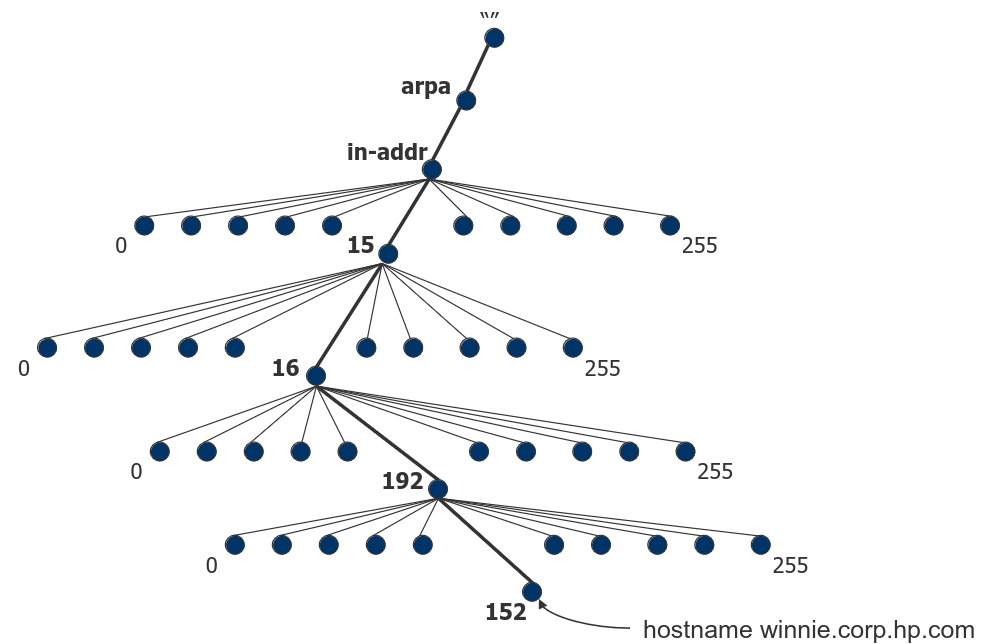
\includegraphics[scale=0.3]{reverselookup.png}
\end{center}
\begin{note}
	This is useful against \textbf{spoofing}: as an example if you get an email and you want to check if the sender is who claims to be, you can do a reverse lookup on the IP of the email server.
\end{note}

\begin{question}[Why does reverse lookup not always work?]
	Because the entries are not always present in the database.
\end{question}

\subsection{Database entries}
A \textbf{resource record} is the entry in the database to get the address or other information of a name. It's composed of a tuple:
\begin{lstlisting}[language=Python]
	(name, TTL, class, type, value)
\end{lstlisting}
\paragraph{TTL} It's the Time To Live: after a certain amounts of seconds the record will be deleted from the cache and updated. With a shorter TTL you have a very updated cache while longer TTL means outdated caches but less requests for the server.
\paragraph{Type} Indicates the type of data to be returned. \textbf{A} is the actual IPv4 address corresponding to the name (\textbf{AAAA} for IPv6). 
\paragraph{Class} Nowadays it's only \textbf{IN} but there were in the past other options for different networks with independent DNS zones.

\begin{observation}[Load balancing]
	DNS is very useful for load balancing: depending on the region when you ask for a DNS entry the answer will be the closest one. It can also be used for \textbf{evil purposes} (censorship, marketing).
\end{observation}

\subsubsection{Name Server}
For each name server of a zone a \textbf{Name Server} record is created in the cache. E.g. when you want to visit \textit{arnold.movie.edu} you may have in cache a NS entry for \textit{movie.edu}.

\subsubsection{CNAME}
A \textbf{CN} record is an optional entry in the database that illustrates aliases on its canonical names. 

\subsubsection{Pointer}
The \textbf{PTR} record provides information for the mapping of an address to names. If you do not have any entry for an IP address you then have to do a reverse lookup. Addresses should refer only to one name.

\subsubsection{Mail Exchanger}
The \textbf{MX} record serves for the controlling of the email routing. It specifies an email server responsible for a domain name with the option to indicate a preference if multiple servers are present (the smallest value is preferred).

\subsection{Protocol}
The resolver software triggers the resolution process and tries first for the cache. Then it sends the request to the local DNS server which is either static (resolv.conf) or dynamic (DHCP). \\
The protocol consists of a single packet used for inquiries and responses:
\begin{center}
	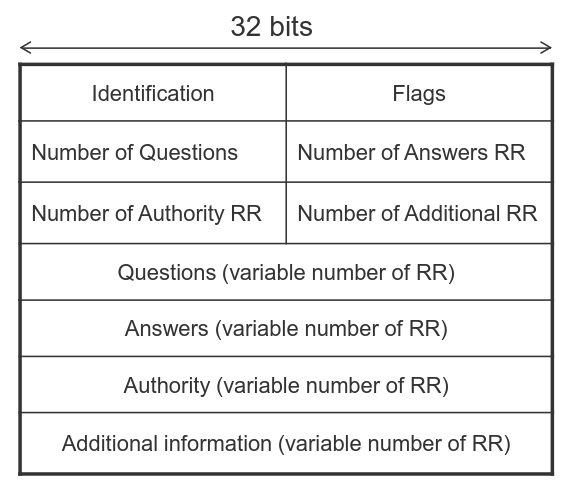
\includegraphics[scale=0.3]{dns.png}
\end{center}
\paragraph{Identification} $16bits$ for the mapping of an inquiry to a response.
\paragraph{Flags} $16bits$ of various flags that indicate if the packet is a request or a response, if it's \textbf{authoritative} or not, if it's \textit{iterative} or \textit{recursive}.
\paragraph{Numbers} These fields indicate the contained number of inquiries responses data records.
\paragraph{Questions} Contains the names to be resolved.
\paragraph{Answers} Resource records to the previous inquiry.
\paragraph{Authority} Contains the ID of the passed responsible NS.
\paragraph{Additional information} If the name searched is only an alias, the belonging resource record for the correct name is placed here.

The packet is sent through UDP on port $53$ and the \textbf{reliability} is only implemented via repeating the requests. Also it is not protected.

\subsection{Scalability}
The scalability is achieved mainly with local caching of recent results. The cache can be in the network and also in the local client.\\
One of the main problem is how long should you keep the entries? You need to achieve both \textbf{consistency} and not doing too many requests. You also need to detect and flush the \textbf{stale entries}. You have to avoid \textbf{cache poisoning}: when a malicious person changes the value in the cache to redirect you to an evil software.
\subsection{Extension}
\subsubsection{Dynamic DNS}
The problem comes up when, as an example, you restart the router and your public IP address is changed (or maybe the ISP changes it every 24 hours). The DDNS allows you to tell the changed IP address.
\subsubsection{Characters}
The original DNS supports only ASCII, so there is an extension for UTF characters.
\subsubsection{DNSSEC}
The \textbf{security} is important because DNS is the most crucial indirection to access the data. Controlling DNS response implies controlling the discovery of the communication endpoints. It may be use in an evil way for political and economical reasons.
\newpage
\section{Email}
\subsection{Introduction}
Email is an example of an application that works on the different layers. It's \textbf{asynchronous}, \textbf{decentralized} (to improve \textit{scaling}), \textbf{client-server} and based on simple ASCII text.
\subsubsection{Motivation}
Email was the first \textit{killer application}. It started in the 1980's with a simple terminal interface, evolving in the 1990's with the \textit{web-mail} and then \textit{mobile email}. Today social network are trying to swallow the email concept.
\subsection{Architecture}
There are two actors involved:
\begin{itemize}
	\item \textbf{User Agent}, with email clients. Runs on the computer of the user and is intermittently on. E.g. Thunderbird or Outlook
	\item \textbf{Message Transfer Agent}: the email servers. They run on a remote machine and stores and forwards on behalf of the User Agents. It's always on
\end{itemize}

\begin{center}
	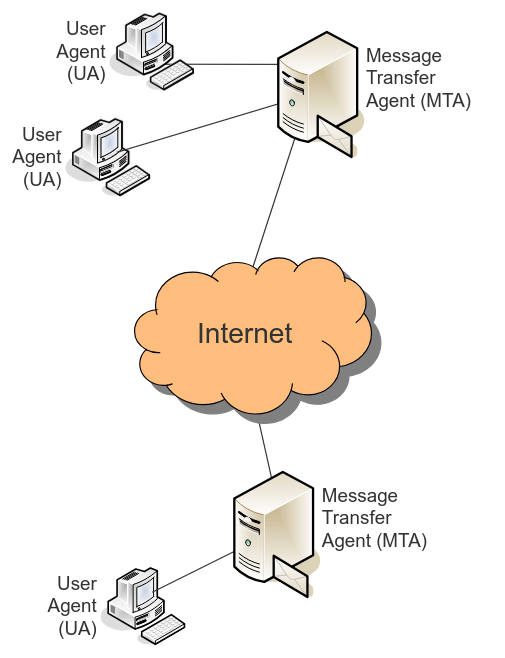
\includegraphics[scale=0.3]{email.png}
\end{center}

\subsection{Message}
Message are viewed as having an \textbf{envelope}, the fundamental part for the delivery, and a \textbf{content}. The latter contains a \textbf{header} with a certain coding and a \textbf{body} consisting of simple characters.

\subsubsection{Envelope}
The envelope is created by the \textbf{MTA} or the \textbf{MSA} and includes all the information for transporting the message. Some information are redundant with the header (like the sending and receiving address) but there are some differences, like when you send a Blind Carbon Copy message.

\begin{note}
	You can't know if the sender is correct. This can be used for evil purposes. The only way to avoid that is by encrypting or signing the email.
\end{note}

\newpage
\subsubsection{Content}
\paragraph{Header} It contains characters with the following syntax:
\begin{lstlisting}
	<key>:<value>
\end{lstlisting}
\paragraph{Body} It's the content of the email. It's separated from the header by a blank line.

Since originally the content could only contain $7bit$ ASCII, \textbf{Multipurpose Internet Mail Extensions} was invented to extend the classical format. It adds additional headers, content types and sub-types:
\begin{itemize}
	\item \textbf{MIME-version}
	\item \textbf{content-description}: string that describes the content of the message
	\item \textbf{content-id}: identifier for the content
	\item \textbf{content-transfer-encoding}: selected coding for the content (BASE64, ASCII)
	\item \textbf{content-type}: specifies the type of the body in the format \textit{type/subtype}, e.g. text, image, audio, video, etc..
\end{itemize}

\subsection{Protocols}
\subsubsection{SMTP}
Simple Mail Transport Protocol delivers the mail to the final inbox. It can't ensure that the message arrives to the final user because it expects the receiver to be always online.\\
It uses \textbf{reliable data transfer} based on TCP on port $25$ and it's \textit{best effort}. It provides \textbf{little security}: no encryption, optional authentication on port $587$ to reach MSA but nothing between MTAs.\\
The protocol follows these steps:
\begin{enumerate}
	\item \textbf{Write} an email, the client formats it and sends it to it's own mail server
	\item The mail server sets up a connection with the receiver's server and \textbf{sends} a copy of the email
	\item The \textbf{receiver}'s server creates the header of the email and places the message in the inbox
\end{enumerate}

\paragraph{Graylisting} A first attempt to block spam. If a combination of IP address of the sender, their email and the receiver's one is seen for the first time, the message is discarded and an error is returned. From the second time on, the message goes through. This is based on the idea that scammers won't send the email twice.

\subsubsection{POP3}
This protocol pulls emails from the server over a connection on port $110$. It's text based and allows basic functionalities such as \textit{logging}, \textit{copying locally} and \textit{deleting} from the server.\\
It works in two phases:
\begin{enumerate}
	\item \textbf{Authorization} phase: \textit{user}name and \textit{pass}word for authentication, either successful or not
	\item \textbf{Transaction} phase: a \textit{list} of the messages and their sizes is provided, then via \textit{retr} its possible to retrieve a message using the number of the list and with \textit{dele} to delete an email.
\end{enumerate}

\begin{note}
	POP3 is heavily limited due to problems with multiple users handling and always-on connections.
\end{note}
\subsubsection{IMAP}
This protocol works on port $143$. In this case the emails remains on the server and may be cached by the client. All the actions are performed on the server. Ideal when you need to access it from different locations.

\subsubsection{HTTP}
The \textbf{webmail} allows the user to interact with emails via WEB. E.g. Gmail or Outlook.
\newpage
\section{HTTP}
HTTP is a protocol that allows the user to request a \textbf{resource} (e.g. HTML page) that is on a server. They may contain references to other resources, therefore creating a \textit{web}, called \textbf{World Wide Web}.
\subsection{History}
The first idea came in 1945 by Vannever Bush, with his \textbf{Memtex}, a desk containing different information categorized accordingly: \textbf{hypertex} context was born. Then in 1962 Doug Engelbart started to work on its actual implementation and by 1989 Tim Berners Lee connected that with TCP/IP and DNS protocols, effectively creating the WWW. \\
Today it gives access to \textbf{intelinked documents} distributed across several computers in the world, using the internet as exchange.

\subsection{Communication}
\subsubsection{HTTP/1}
The standard way of communicating is between a \textbf{client} (e.g. Firefox, Chrome) and a \textbf{web server} (e.g. Apache, Nginx).\\
The communication is handled by the HTTP protocol (usually on port $80$). It's a text based \textbf{request/response} protocol.\\
It was \textbf{stateless} until version 2. This means that the server maintains no information about previous requests and thus the specification of the context is needed every time.\\

\paragraph{Request} HTTP requests follow the \textbf{REST} API principle, allowing for performance, scalability, simplicity, modifiability, portability and reliability. The resources are retrieved via a \textbf{URL}

\begin{center}
	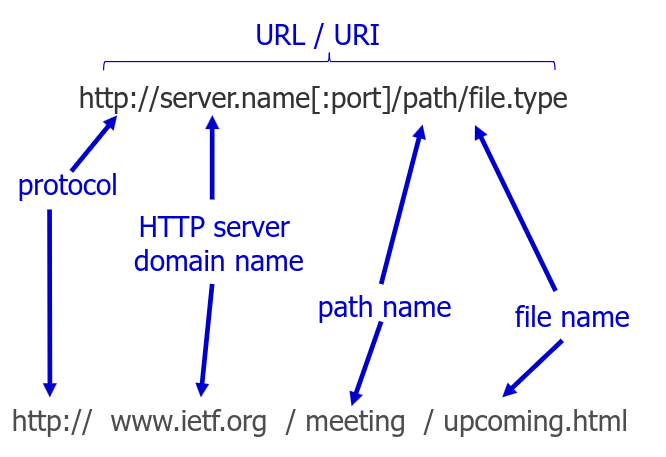
\includegraphics[scale=0.3]{url.png}
	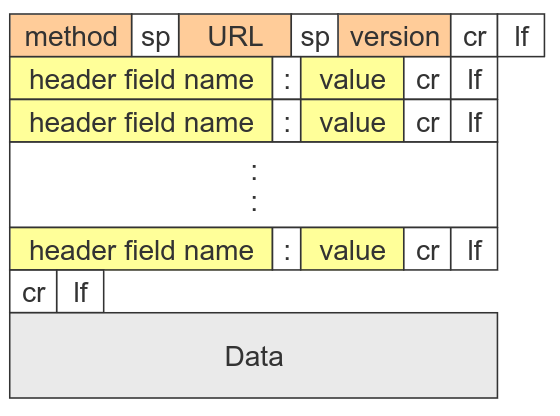
\includegraphics[scale=0.3]{httpreq.png}
\end{center}

\noindent The specified commands that can be used with a URL are:
\begin{itemize}
	\item \textbf{GET}: load a web page
	\item \textbf{HEAD}: load only the header of the web page, used for \textit{debugging}
	\item \textbf{PUT}: store a page on the web server
	\item \textbf{POST}: append something to the request passed to the web server
	\item \textbf{DELETE}: delete a web page
\end{itemize}

\newpage
\paragraph{Response}  The HTTP response contains the protocol used, the header lines and the \textbf{status code} , that can be:
\begin{itemize}
	\item \textbf{1xx}: only for information
	\item \textbf{2xx}: successful inquiry
	\item \textbf{3xx}: further activities are necessary
	\item \textbf{4xx}: client error (syntax)
	\item \textbf{5xx}: server error
\end{itemize}
\begin{center}
	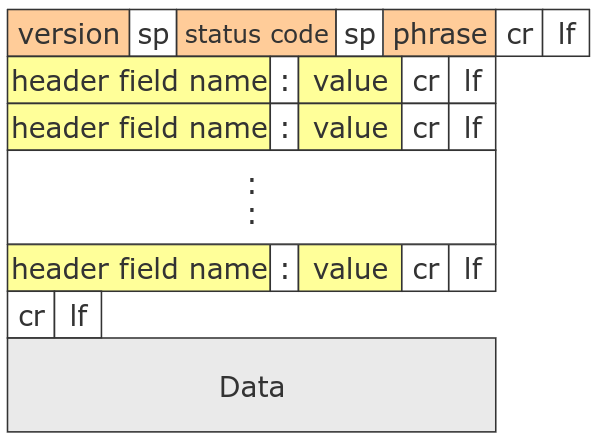
\includegraphics[scale=0.3]{httpresp.png}
\end{center}

\subsubsection{Web Sockets}
HTTP first problem is that the client needs to poll explicitly for content, causing a huge \textbf{overhead}. Thus Web Sockets were created: they allow a full duplex communication between the server and the client without the need of HTTP. It uses the same ports and it's set up using an HTTP request to "upgrade", which is then answered with a "switching protocol" response.

\subsubsection{WebRTC}
HTTP second problems is to enable communications between multiple browsers without creating a web server for each one of them. WebRTC implements a P2P communication that provides functions to establish media and data exchange, e.g. for videoconferencing.

\subsubsection{HTTP/2}
The second version of HTTP is \textbf{binary} instead of text based. It is fully \textbf{multiplexed}, associating requests and response and allowing a bi-directional stream. Therefore it can use only one connection while still granting \textbf{parallelism}. Furthermore it uses \textbf{header compression} to reduce overhead and allows server to push responses into client caches, reducing the number of requests to render web pages.
\begin{center}
	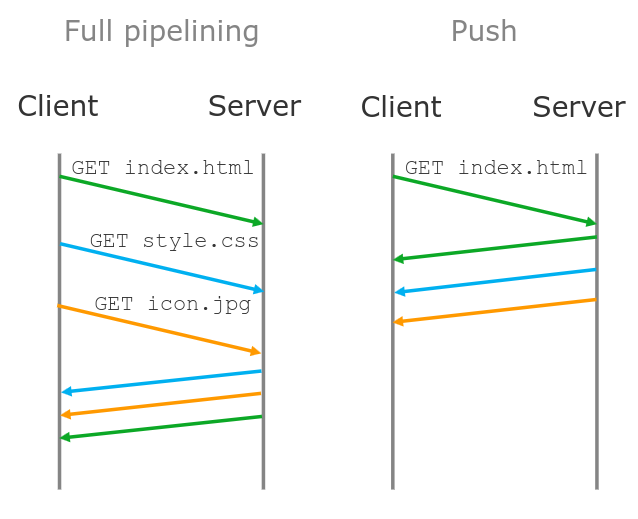
\includegraphics[scale=0.25]{http2.png}
\end{center}
\subsubsection{HTTP/3}
This version uses \textbf{QUIC} protocol over UDP instead of TCP and TLS for security, avoiding \textit{head of line} blocking.

\subsection{Cookies}
The main problem with HTTP is that it's \textbf{stateless}, this meaning that after every request/reply the web server forgets everything. While this is not a problem for simple browsing, it means that we cannot store user content to personalize the experience.\\
The solution is the \textbf{cookies}: tags stored in the web browser and set by the server so that they can be sent again to allow the latter to identify the client.\\
\subsubsection{Structure}
Cookies are stored as name-value pairs defined by the server. They can have optional parameters such as an \textbf{expiry date}.
\begin{center}
	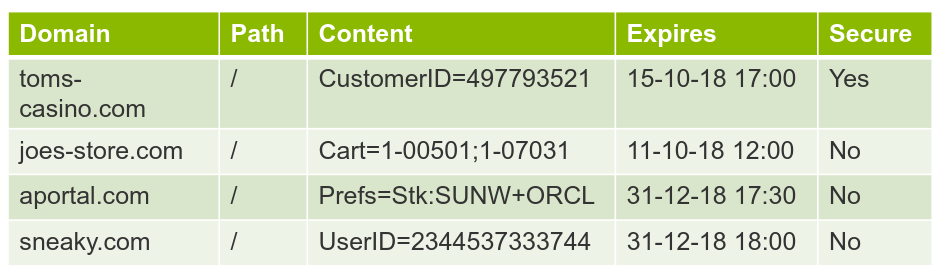
\includegraphics[scale=0.4]{cookies.png}
\end{center}

\subsubsection{Pros and cons}
They enable \textbf{authorization}, shopping carts, recommendations and \textbf{user session state} (e.g. for web mail). The biggest problem is about \textbf{privacy}: cookies are identified by \textbf{Etags}, an opaque identifier for a specific version of a resource, and can be used to track users.

\subsection{Proxy}
A \textbf{proxy} is an intermediate cache between multiple clients and a server. The main goal is to have a more \textbf{efficient} page loading, improving \textbf{scalability}. It temporarily stores the pages loaded by the browsers: if the client requests it and it hasn't changed yet, it's loaded from the proxy, otherwise a new request to the server is made and the cache is updated.\\
It can also enable support for protocols such as FTP or Telnet without the need for a new browser implementation.\\
It can also work as a \textbf{firewall}. 

\subsection{Scaling}
To handle huge loads (top 1000 websites) we use \textbf{3-tier} architecture, which separates the web server in \textbf{presentation servers}, \textbf{logic servers} and \textbf{database storage}. 
\begin{center}
	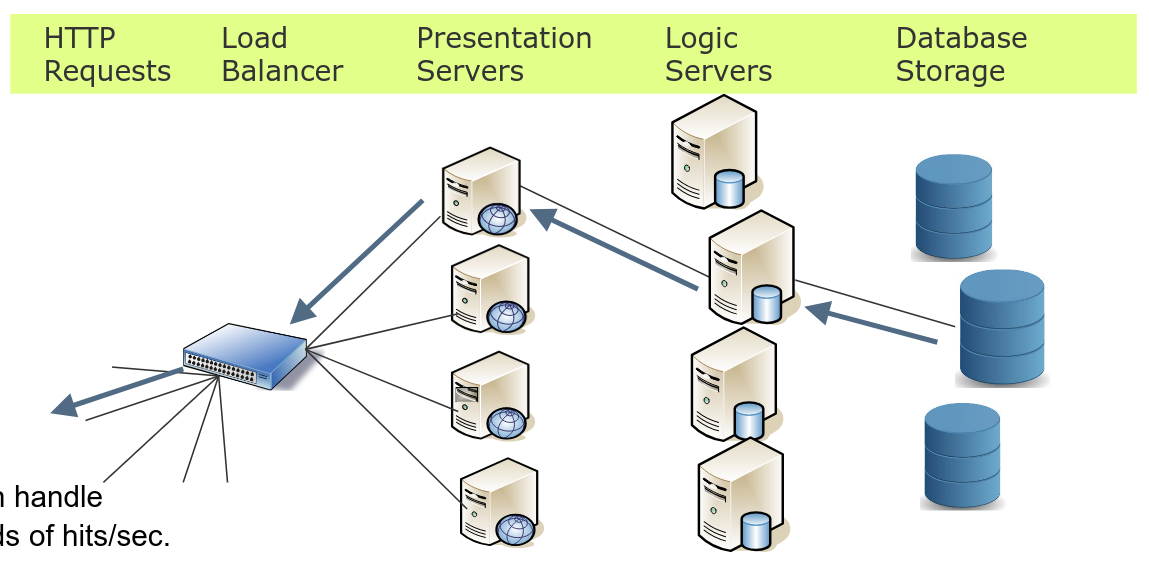
\includegraphics[scale=0.25]{3tier.png}
\end{center}
If, instead, we want to deal with medium and small web servers, we usually virtualize a lot of them on a single machine and we do the multiplexing with the server URL field in HTTP.

\subsection{DNS}
It's possible to use DNS over HTTP by sending a request (either \textit{GET} or \textit{POST}) to the DNS server. It improves privacy and security but the user looses control.
% !TeX spellcheck = en_US
\newpage
\section{SNMP}
The Simple Network Management Protocol allows the management of devices and services using a simple datagram service with a \textbf{client-server} architecture:
\begin{itemize}
	\item \textbf{Agent}: process continuously running on each managed node collecting information
	\item \textbf{Manager}: process running intermittently on a management workstation that requires information about the devices in the network
\end{itemize}
There may also be a \textbf{proxy agent} that integrates non-SNMP capable systems
\subsection{Motivation}
If we have problems in the network we need a \textbf{management tool} to be able to correctly identify them and their causes. In particular the tool needs to manage:
\begin{itemize}
	\item \textbf{Performance}: measure and analyze network performance to provide good network service
	\item \textbf{Configuration}: monitor or modify configuration settings or HW or SW elements
	\item \textbf{Accounting}: measure network utilization parameters per user or group of users
	\item \textbf{Fault}: detect, log, notify users and automatically fix problems while running
	\item \textbf{Security}: control access to network resources according to local guidelines to avoid sabotage and unauthorized access to sensitive information
\end{itemize}

\begin{observation}
	It should be achieved \textbf{remotely} over the existing network, meaning a protocol above IP.
\end{observation}

\subsubsection{Goals}
The main goals of network management are:
\begin{itemize}
	\item \textbf{Monitoring} HW equipment
	\item \textbf{Statistics} of network usage
	\item Remote \textbf{diagnostics}
	\item \textbf{Protected} and \textbf{safe} networking
	\item \textbf{Efficient} internetworking
	\item Simple model of \textbf{network status}
	\item Gather data for \textbf{network planning}
\end{itemize}

\subsection{Overview}
A network management framework is based on three building blocks:
\begin{itemize}
	\item \textbf{SNMP}: defines \textbf{format of messages} exchanged by management systems and agents and \textbf{basic operations}
	\item \textbf{SMI}: Structure of Management Information specifies how the monitored information is structured, defining the objects that SNMP protocol accesses over the network
	\item \textbf{MIB}: Management Information Base describes the concrete managed objects and is an open concept for data storage. It may be public (RFC) or proprietary.
\end{itemize}

\subsubsection{History}
There have been three major versions of SNMP during history:
\begin{itemize}
	\item \textbf{SNMPv1}, 1998, was designed originally as an interim solution but became the standard. It had very weak security model with complex bulk requests but was simpler than CMIS/CMIP
	\item \textbf{SNMPv2}, which was then split in
	\begin{itemize}
		\item \textit{SNMPv2u}: user-based security
		\item \textit{SNMPv2*}: user-based security and additional features
		\item \textit{SNMPv2c}: without security but with \textit{GetBulk} operation
	\end{itemize}
	\item \textbf{SNMPv3}, the current one, that provides an advanced security model: now each message has security parameters, integrity and authentication.
\end{itemize}

\subsection{Managed objects}
An \textit{agent} monitors the network resources that are abstracted as \textbf{managed objects}. Each one has a \textbf{unique ID} and a \textbf{name} and models various property of the resource. Its standard components are:
\begin{itemize}
	\item \textbf{Common prefix} + \textbf{Unique name}: e.g. \textit{iso.org.dod.internet.mgmt.mib.system.sysDescr}
	\item \textbf{Syntax}: simple data types \textit{integer}, \textit{string} and \textit{array}
	\item \textbf{Access rights}: \textit{read-only} or \textit{read-write}
	\item \textbf{Status}: \textit{mandatory} or \textit{optional}
\end{itemize}

\begin{wrapfigure}[7]{r}{3cm}
	\vspace{-1.5cm}
	\begin{center}
		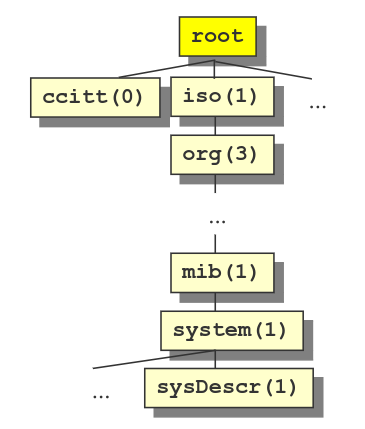
\includegraphics[width=3cm]{objs}
	\end{center}
\end{wrapfigure}
\paragraph{MIB}
The Management Information Base is a distributed virtual database that hosts the collection of managed objects that belong to the same context. It defines the capabilities of the device that can be managed.\\
In particular \textbf{MIB-2} defines the generics for all manageable internet devices. Its prefix is \textit{iso(1).org(3).dod(6).internet(1).mgmt(2).mib2(1)}. Some examples are \textit{batteryAgingNotification} with OID \textit{1.3.6.1.2.1.233.0.5} and \textit{sysLocation} with \textit{1.3.6.1.2.1.1.6}.\\
Another specific MIB is \textbf{RMON} for Remote Monitoring, it has more advanced functions such as gathering of statistics, alarms, events, on-board evaluations.
\paragraph{MIT}
Each managed object has a unique position in the Management Information Tree, thus providing a unique reference.

\begin{center}
	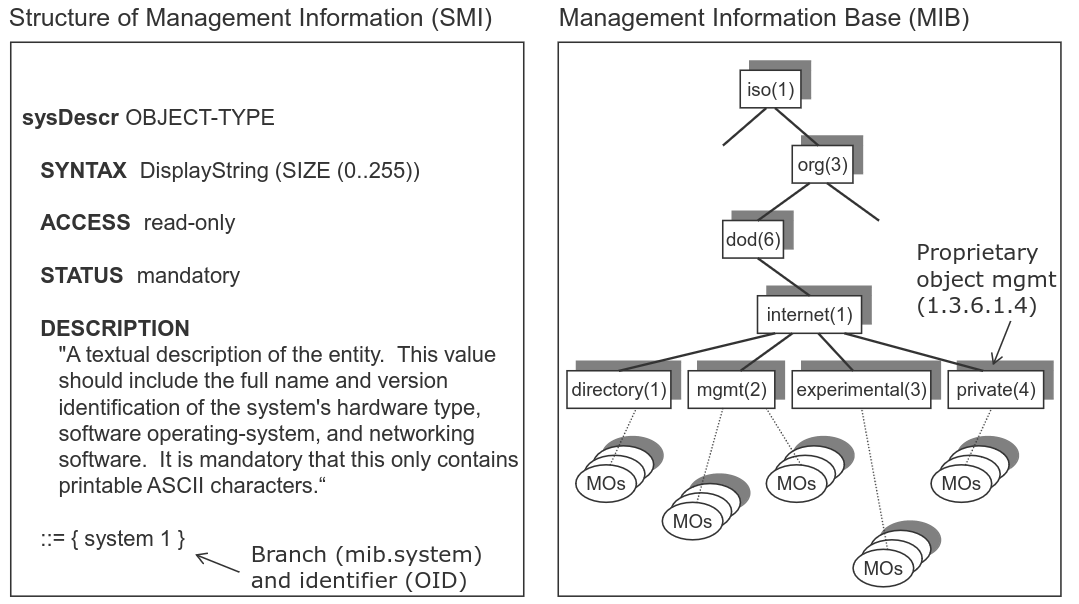
\includegraphics[scale=0.35]{mibsmi}
\end{center}

\subsubsection{Encoding}
Since different systems use different data representation, it's necessary to recode data while maintaining its meaning. To do that the message is first composed in ASN.1 syntax and then transferred using BER.
\paragraph{ASN.1}
Abstract Syntax Notation One is an ISO standardized language for representation-independent specification of data types. It's used in SNMP to describe managed objects. It consists of:
\begin{itemize}
	\item \textbf{Elementary} types, such as \textit{boolean}, \textit{integer}, \textit{bitstring}, $\ldots$
	\item \textbf{Structured} types:
	\begin{itemize}
		\item \textbf{Sequence}: ordered list of data types
		\item \textbf{Set}: unordered set of data types
		\item \textbf{Sequence Of}: like \textit{array} in C
		\item \textbf{Set Of}: unordered set of elements from the same data type
		\item \textbf{Choice}: like \textit{union} in C
	\end{itemize}
\end{itemize}
\begin{example}
	Some types defined by ASN.1:
	\begin{lstlisting}
		- INTEGER
			- signed 32-bit int
		- OCTET STRING
		- OBJECT IDENTIFIER (OID)
	\end{lstlisting}
	and some defined by SMI:
	\begin{lstlisting}
		- IpAddress
			- OCTET STRING of size 4, in network byte order
		- Counter
			- unsigned 32-bit int (rolls over)
		- Gauge
			- unsigned 32-bit int (will top out and stay there)
		- TimeTicks
			- unsigned 32-bit int (rolls over after 497 days)
		- Opaque
			- used to create new data types not in SNMPv1
		- DateAndTime, DisplayString, MacAddress, PhysAddress, TimeInterval, TimeStamp, TruthValue, VariablePointer
			- textual conventions used as types
	\end{lstlisting}
\end{example}

\paragraph{BER}
ASN.1 content is then converted into smaller binary data that follows the Basic Encoding Rules, like source code is converted to machine code.
\begin{center}
	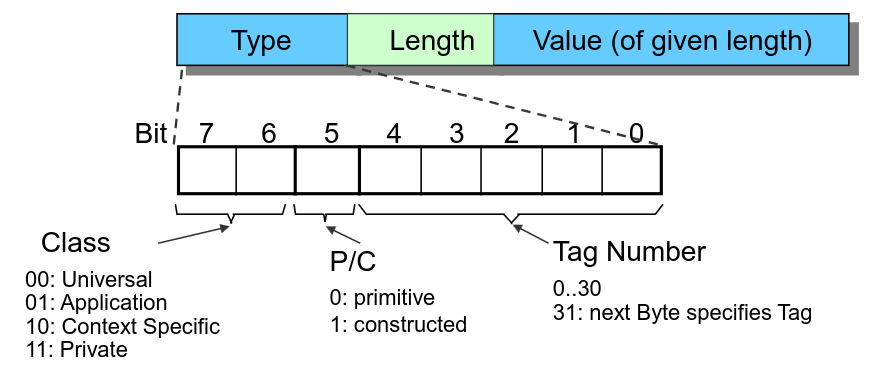
\includegraphics[scale=0.4]{ber}
\end{center}

\subsection{Operations}
SNMP has five main operations:
\begin{itemize}
	\item \textbf{GetRequest}, \textbf{GetNextRequest}, \textbf{SetRequest} and \textbf{GetResponse} that are initiated by the SNMP manager
	\item \textbf{Trap} that allows an agent to push information to the manager
	\item \textbf{GetBulkRequest} is a series of \textit{GetNextRequest}
\end{itemize}
\begin{center}
	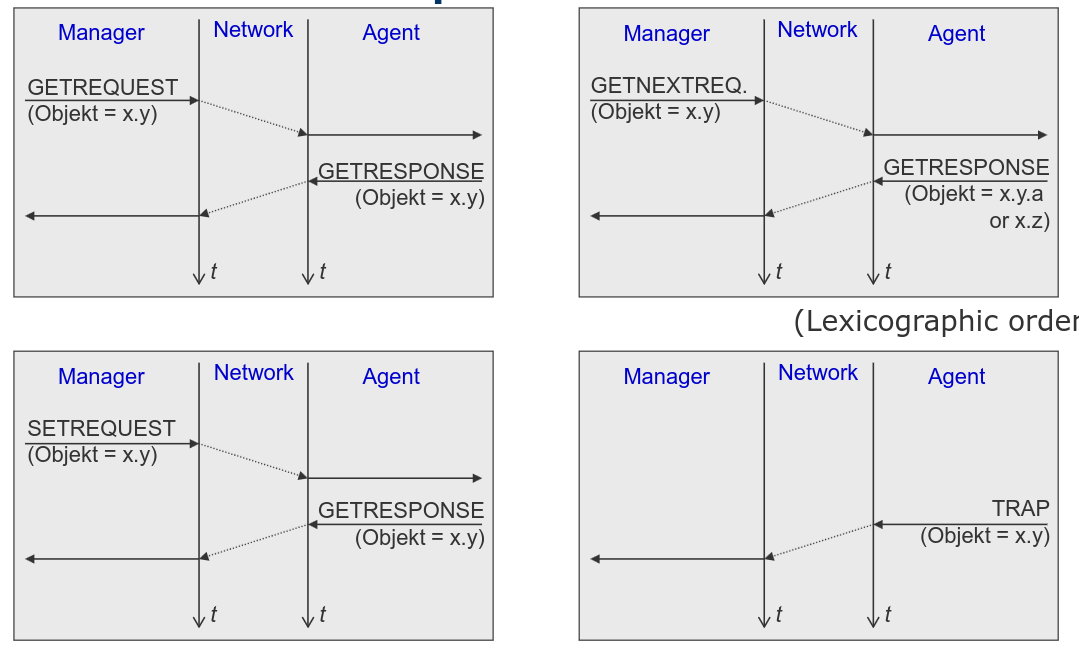
\includegraphics[scale=0.4]{ops}
\end{center}
SNMP works on a well-known UDP port: 161 for everything except of \textit{Trap} that is on 162.

\subsubsection{Packet format}
\begin{wraptable}[10]{r}{4cm}
	\vspace{5.7cm}
	\scalebox{1}{
		\begin{tabular}{c|c}
			0 & noError \\
			1 & tooBig \\
			2 & noSuchName \\
			3 & badValue \\
			4 & readOnly \\
			5 & genErr
		\end{tabular}
	}
\end{wraptable}
The packet is divided in:
\begin{center}
	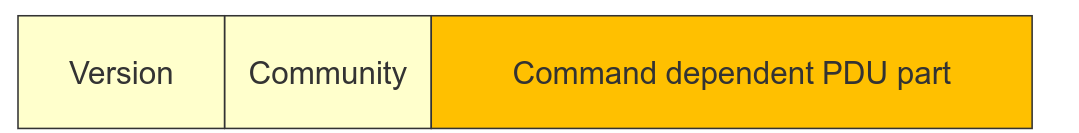
\includegraphics[scale=0.25]{packet1}
\end{center}
\begin{itemize}
	\item \textbf{Version}: version number of SNMP
	\item \textbf{Community}: string used for authentication, transmitted in plain text
	\item Command dependent\textbf{PDU}:
	\begin{center}
		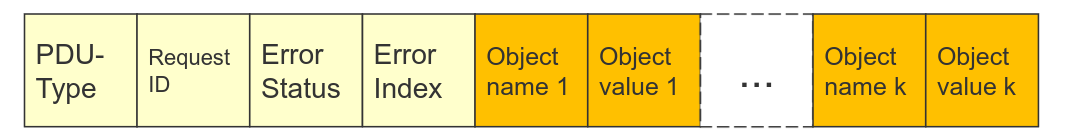
\includegraphics[scale=0.25]{packet2}
	\end{center}
	\begin{itemize}
		\item \textbf{PDU-Type}
		\item \textbf{Request Id}: identification of pending request
		\item \textbf{Error Status}, based on the result of the query
		\item \textbf{Error Index}: reference to the variable binding pair that caused the failure
		\item Variable length list of pairs of (Object Name, Object Value)
	\end{itemize}
\end{itemize}

\subsection{Tools}
There are different tools:
\begin{itemize}
	\item \textbf{Command line} like \textit{snmpget}, \textit{snmpnext}, etc that allows the generation and decoding of SNMP data units and sometimes also support for MIB files
	\item \textbf{MIB Browser}
	\item \textbf{Management Platforms} like \textit{CiscoWorks} and \textbf{Nagios} (open source)
\end{itemize}
All of the tools need to do the \textbf{discovery} and \textbf{polling} of the network topology through ICMP, SNMP and HTTP, among diffent devices with common interfaces but also vendor specific functionalities.

\subsection{NETCONF}
SNMP is used for monitoring only and therefore a tool for configuration is needed. NETCONF is based on XML and messages are exchanged through a secure transport protocol. The included operations are:
\begin{itemize}
	\item \textbf{get}: retrieve running configuration and device state information
	\item \textbf{get-config}: retrieve all or of a specified configuration datastore
	\item \textbf{edit-config}: edit a configuration datastore by creating, deleting, merging or replacing content
	\item \textbf{copy-config}: copy an entire configuration datastore to another configuration datastore
	\item \textbf{delete-config}: delete a configuration datastore
	\item \textbf{lock}: lock an entire configuration datastore of a device
	\item \textbf{unlock}: release a configuration datastore lock previously obtained with the \textit{lock} operation
	\item \textbf{close-session}: request graceful termination of a NETCONF session
	\item \textbf{kill-session}: force the termination of a NETCONF session 
\end{itemize}

An extension of NETCONF is \textbf{RESTCONF}, which allows accessing data defined in \textbf{YANG}. YANG (Yet Another Next Generation) is a data modeling language for the definition of the data. It can be used for configuration data, status of devices, events or notification. It's protocol independent but can be converted into XML or JSON. It's \textbf{modular} and represents data structures as XML tree, with many data types.
\subsubsection{NETCONF vs SNMP}
Let's analyze the main differences:
\begin{itemize}
	\item \textbf{Security}: NETCONF offers more granular and flexible access control mechanism, it runs over SSH or TLS (RESTCONF on HTTPS), while SNMP lacks proper encryption and authentication
	\item \textbf{Structure}: NETCONF uses structured data models to define the configuration and operational state of network devices, a clear and standardized way that reduces misconfigurations. On the other hand, SNMP is less structured and less intuitive (tree structure), often requiring complex OIDs and more prone to errors
	\item \textbf{Functionality}: SNMP can only retrieve device data while NETCONF can also modify or replace configurations
\end{itemize}
% !TeX spellcheck = en_US
\newpage
\section{Physical}
In the network we have the \textbf{hosts}, end systems hosting user applications, and the \textbf{routers}, intermediate systems providing network connectivity.
\begin{center}
	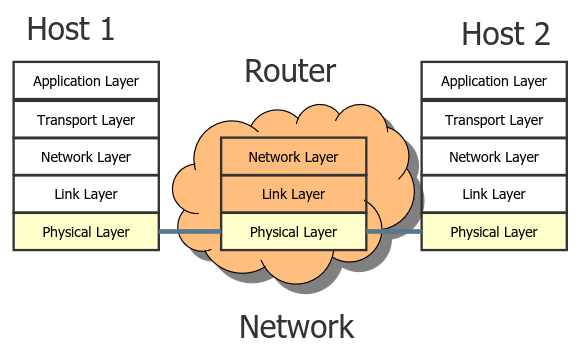
\includegraphics[scale=0.35]{ph}
\end{center}
The hosts have the full stack implementation while the routers only up to the Network Layer.
\subsection{Signals}
\begin{definition}[Signal]
	A signal is the physical representation of the data. It can be:
	\begin{itemize}
		\item \textbf{Analogue}: sequence of \textit{continuous} values
		\item \textbf{Digital}: sequence of \textit{discrete} values
	\end{itemize}
\end{definition}

Data is converted to signal which is then sent over the \textbf{transmission channel}, which is composed by \textbf{access points} and a \textbf{physical medium} (e.g. copper).
\begin{center}
	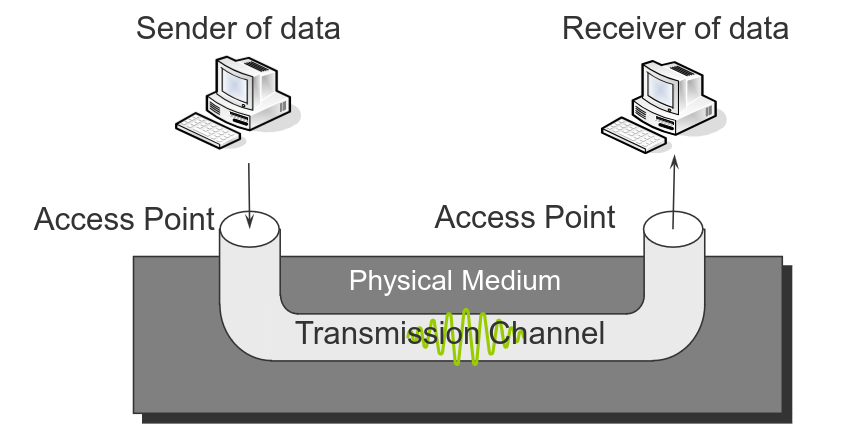
\includegraphics[scale=0.3]{phtr}
\end{center}
Since computers deal with digital signals, transmitting one bit via at a time a given medium, they need:
\begin{itemize}
	\item \textbf{Quantization}: convert from digital signal to analog signal and vice versa
	\item \textbf{Sampling}: must rely on periodical measurements of the physical medium
\end{itemize}
\begin{center}
	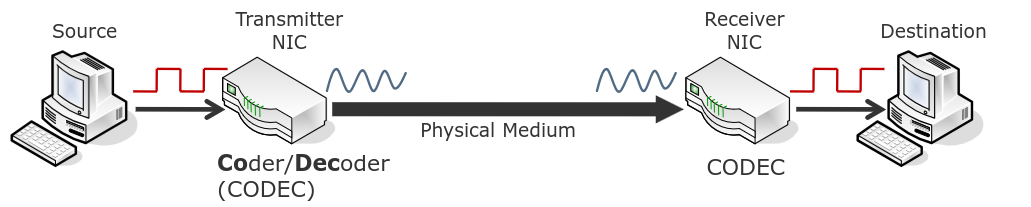
\includegraphics[scale=0.3]{codec}
\end{center}

\begin{observation}
	We have different challenges during the transmission of data:
	\begin{itemize}
		\item \textbf{Internal}: \textbf{collision} and \textbf{synchronization}
		\item \textbf{External}: \textbf{noise}
	\end{itemize}
\end{observation}

\newpage
\subsubsection{Periodic signal}
Periodic signals are the simplest signals. They take the following parameters:
\begin{itemize}
	\item \textbf{Period} $T$
	\item \textbf{Frequency} $f=\frac{1}{T}$
	\item \textbf{Amplitude} $S(t)$
	\item \textbf{Phase} $\varphi$
\end{itemize}

\begin{example}
	Some examples of signals:
	\begin{figure}[!h]
		\hfil
		\subfigure[Sine wave]{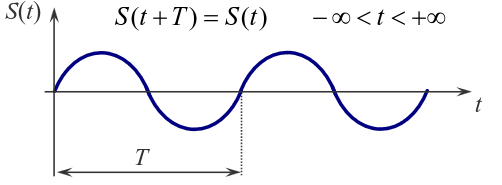
\includegraphics[scale=0.25]{sine}}
		\hfil
		\subfigure[Phase]{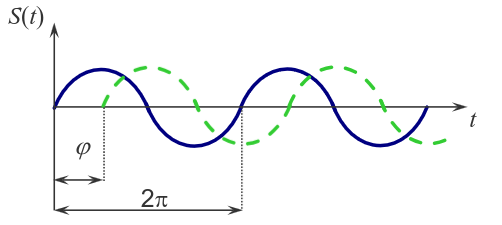
\includegraphics[scale=0.25]{phase}}
		\hfil
		\subfigure[Square wave]{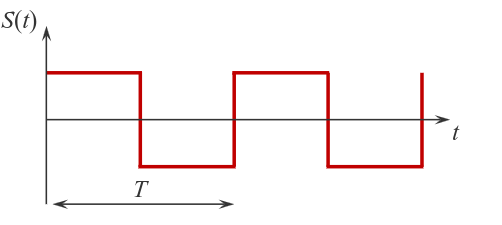
\includegraphics[scale=0.25]{square}}
	\end{figure}
\end{example}

\paragraph{Fourier Analysis} Like the composition of functions, it's possible to \textbf{compose} signals, generating new ones. In fact, per the \textbf{Fourier Analysis}, any period function can be constructed as the sum of a number of sines and cosines, resulting in a \textbf{Fourier Series}.
\begin{equation}
	g(t)=\frac{1}{2} c + \sum_{n=1}^{\infty} a_n \sin(2\pi nft) + \sum_{n=1}^{\infty}b_n \cos(2\pi nft)
\end{equation}
\textbf{Fourier Transform} is a mathematical transformation used to transform signals between time domain and frequency domain. Exists also in two dimensional space.
\paragraph{Distortion} If all Fourier components were equally diminished the resulting signal would be reduced in amplitude but not distorted. Unfortunately all transmission facilities diminish different components by different amounts, introducing \textbf{distortion}.

\paragraph{Frequency domain} The frequency domain is described by:
\begin{itemize}
	\item \textbf{Spectrum}: the range of frequencies a signals consists in
	\item \textbf{Bandwidth}: width of the \textit{spectrum}. In theory many signals have infinite bandwidth. The \textbf{effective bandwidth} is the narrow band of frequencies where most of the energy is contained.
\end{itemize}

\begin{example}
	In the following signal we have a \textbf{spectrum} from $f$ to $3f$ and a \textbf{bandwidth} of $2f$.
	\begin{figure}[!h]
		\hfil
		\subfigure[Time domain]{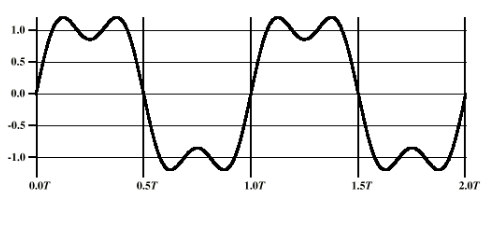
\includegraphics[scale=0.3]{time}}
		\hfil
		\subfigure[Frequency domain]{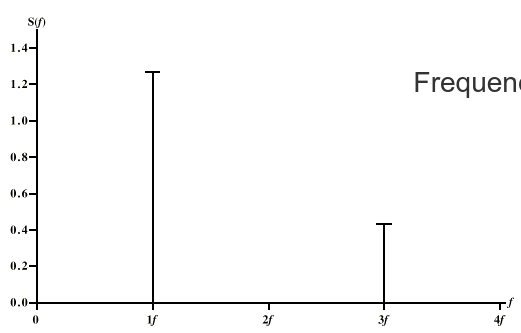
\includegraphics[scale=0.3]{freq}}
	\end{figure}
\end{example}

\subsubsection{Bandwidth}
We have two possible digital signal:
\begin{itemize}
	\item \textbf{Binary}: two possible values, $0$ and $1$
	\item \textbf{Multilevel}: more than two possible values (e.g. ternary, quaternary)
\end{itemize}
\begin{definition}[Symbol rate]
	Number of physical signaling events per unit of time on the transmission medium. The unit of measure is a \textbf{baud}.
\end{definition}
\begin{definition}[Data rate]
	Rate of bits decoded from symbol rate per unit of time. The unit of measure is $\frac{\text{bit}}{s}$. There are two cases:
	\begin{itemize}
		\item \textbf{Binary} signals with frequency $v$, each signaling event codes one bit
		\begin{equation*}
			\text{Data rate}=v
		\end{equation*}
		\item \textbf{Multilevel} signals with $n$ possible values
		\begin{equation*}
			\text{Data rate}=v \cdot \log_2(n)
		\end{equation*}
	\end{itemize}
\end{definition}

\begin{example}
	In this image we have a square wave with a negative ($0$) and a positive ($1$) pulse 
	\begin{center}
		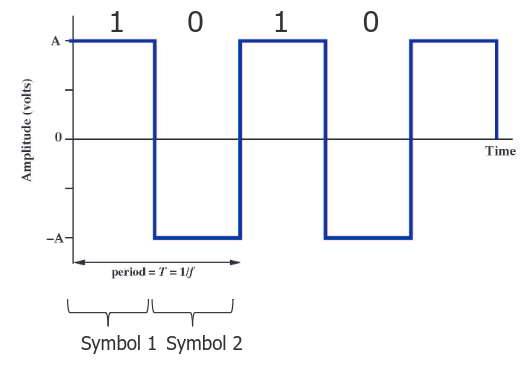
\includegraphics[scale=0.3]{bitrate}
	\end{center}
	The duration of a symbol is $\frac{1}{2} \cdot T = \frac{1}{2f}$, hence the \textbf{symbol rate} (which in this case is equal to the \textbf{data rate}) is $2f$ bits per second.
\end{example}

\begin{definition}[Bandwidth]
	The bandwidth of the medium is the highest $f_H$ minus lowest $f_L$ frequency which can be transmitted over this medium (in \textit{Hz}). $f_0$ is the center frequency.
	\begin{center}
		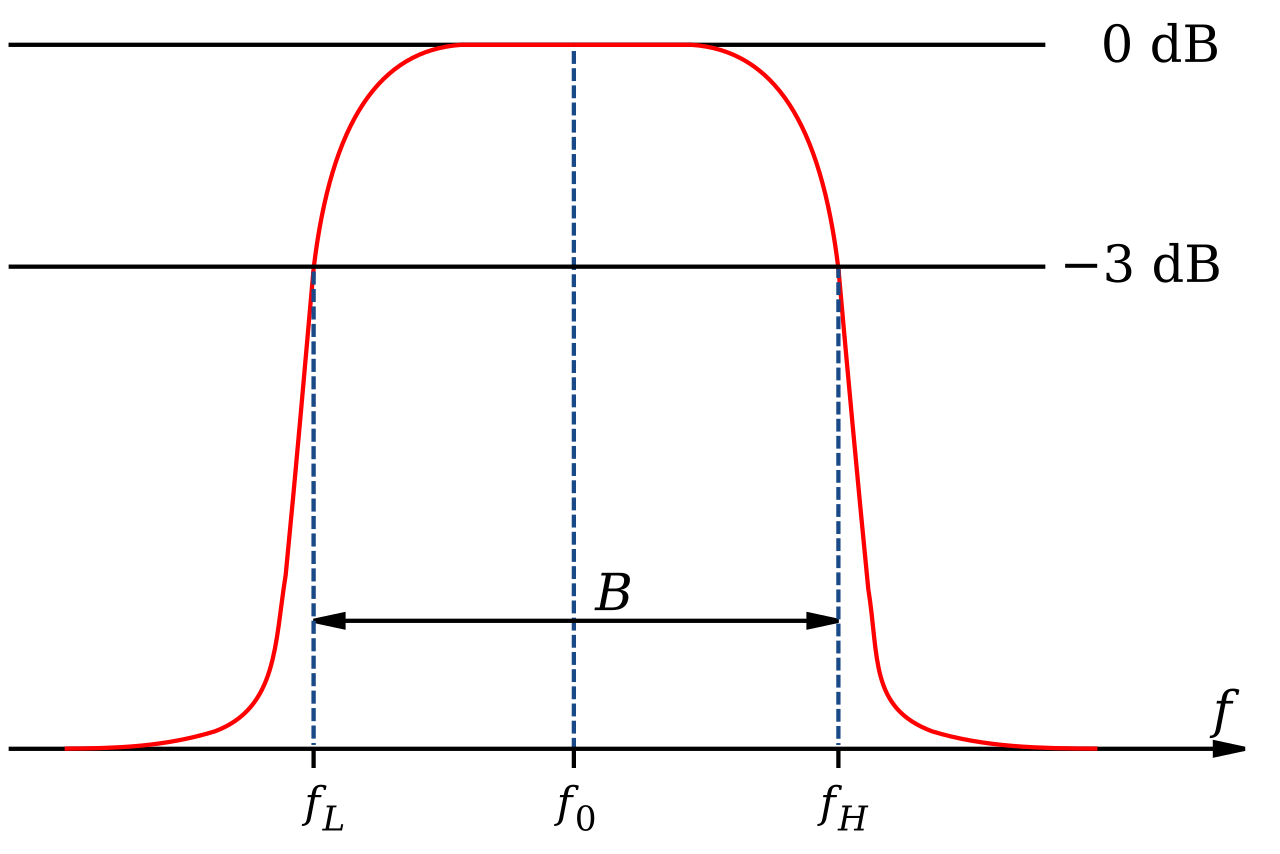
\includegraphics[scale=0.1]{bw}
	\end{center}
\end{definition}
A \textbf{square wave} is composed of an infinite number of \textbf{harmonics}, where the amplitude of the $k$th one is $\frac{1}{k}$.
\begin{equation}
	s(t)=A \cdot \frac{4}{\pi}\cdot\sum_{k=1, k \text{ odd}}^{\infty}\frac{1}{k}\sin(2\pi kft)
\end{equation}
While theoretically we would need an infinite bandwidth to get a square wave, the medium limits the number of harmonics.
\subsection{Transmission}
The fundamental problem of communication consists in reproducing on one side exactly or approximated a message selected on the other side. The ideal transmission would be a square wave while the actual one is an approximation.\\
To get from an analog to a digital signal, there are two main operations:
\begin{itemize}
	\item \textbf{Quantization}: from a continuous value we get a discrete one with an error
	\item \textbf{Sampling}: periodical measures at a given rate with an interval $T$
	\begin{theorem}[Nyquist Sampling Theorem]
		To allow the reconstruction of the original analog signal it is sufficient that the sampling frequency $f_s$ is such that
		\begin{equation}
			f_s > 2W
		\end{equation}
		where $W$ is the bandwidth in Hz.
	\end{theorem}
\end{itemize}

\begin{center}
	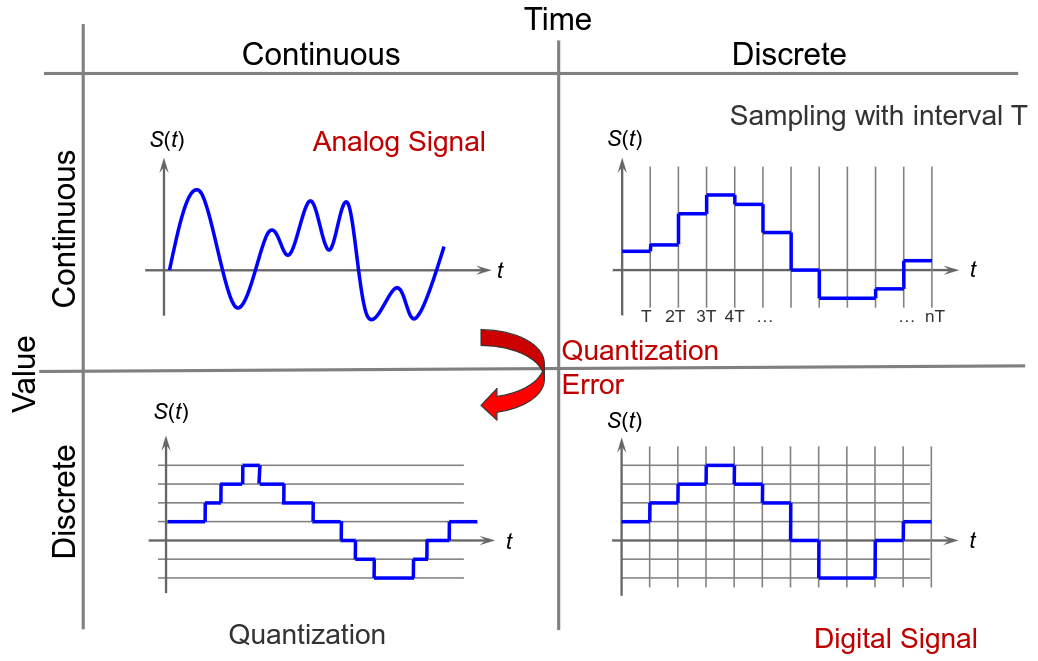
\includegraphics[scale=0.3]{andig}
\end{center}
To get an analog signal from a digital one we perform the \textbf{coding} operation, where the quantization intervals are assigned to a binary code and then transmitted.

\subsubsection{Channel capacity}
To define the \textbf{capacity} of an analog physical channel, we need to consider that there is always some \textbf{noise}. This means that the capacity will be \textbf{finite} and will depend on several parameters, usually:
\begin{itemize}
	\item \textbf{Additive}: the noise value is added to the signal and that's what the receiver gets
	\item \textbf{White noise}: independent, random noise values with constant spectral density
	\item \textbf{Gaussian}: probability distribution of the amplitude of random noise values
\end{itemize}
While on the analog signals noise will cause degradation of the quality, on digital ones it causes \textbf{bit errors}. It is possible to reduce the effect of noise by boosting signal amplitude, but requires energy and causes more interferences.\\ \textbf{Transmission impairments} essentially come from:
\begin{itemize}
	\item Signal \textbf{attenuation} and \textbf{attenuation distortion}
	\item \textbf{Delay distortion}
	\item \textbf{Noise}
	\begin{itemize}
		\item \textit{Thermal} noise
		\item \textit{Intermodulation} noise
		\item \textit{Crosstalk}
		\item \textit{Impulse} noise
	\end{itemize}
\end{itemize}
\newpage
\begin{definition}[BER]
	Bit Error Rate is a metric for bit errors. It depends on the \textbf{environment}, on the \textbf{communication medium} and the \textbf{length} of the transmission line (higher frequencies attenuated stronger than lower, different frequencies have different speed).
	\begin{equation}
		\text{BER} = \frac{\text{Number of erroneous bits}}{\text{Number of transmitted bits}}
	\end{equation}
\end{definition}
\begin{theorem}[Shannon Theorem]
	A channel with $W$ bandwidth, $P$ average signal power and $N$ average noise power has a maximum data rate of:
	\begin{equation}
		\text{maximum data rate} = W \cdot \log_2(1+\underbrace{\frac{P}{N}}_{\text{SNR\footnotemark}})
	\end{equation}
\end{theorem}

\footnotetext{Signal to Noise Ratio}

\noindent Even if we don't consider noise, throughput is still \textbf{finite} due to:
\begin{itemize}
	\item \textbf{Quantization} at the transmitter and \textbf{discrete levels} of the signals
	\item \textbf{Sampling} at the receiver
\end{itemize}
While Shannon Theorem gives us an upper bound for the data rate, we can use Nyquist theorem to calculate the amount of discrete signals needed to achieve that.
\begin{theorem}[Nyquist theorem]
	Given a channel of $W$ bandwidth and $n$ discrete levels of the signal, the maximum data rate is
	\begin{equation}
		\text{maximum data rate} = 2W \cdot \log_2(n)
	\end{equation}
\end{theorem}

\subsection{Data encoding}
To transmit individual bits there are two options:
\begin{itemize}
	\item \textbf{Baseband}: the original data is transmitted "as is" over the medium, requiring \textbf{data encoding}
	\item \textbf{Broadband}: the data is transmitted by \textbf{modulating} it onto a \textbf{carrier} analog signal
\end{itemize}
A data encoding technique needs:
\begin{itemize}
	\item \textbf{Robustness}: tolerance to distortion
	\item \textbf{Efficiency}: high transmission rate, achieved using coded words (binary, ternary, quaternary)
	\item \textbf{Synchronization} with receiver: less opportunities for out-of-sync. Achieved by frequent changes of voltage level regarding to a fixed cycle. Needs to avoid direct current: positive and negative signals should alternatively arise. Bipolar/Unipolar encoding.
\end{itemize}

\subsubsection{NRZ}
Non Return to Zero is a simple approach where $1$ is coded with a positive voltage ($+5V$) and $0$ 	as a negative one ($-5V$). It's very \textbf{simple} and the smaller the clock pulse, the higher the data rate. It's prone to \textbf{loss of synchronization} and has \textbf{direct current} during long sequences of the same bit.
\begin{center}
	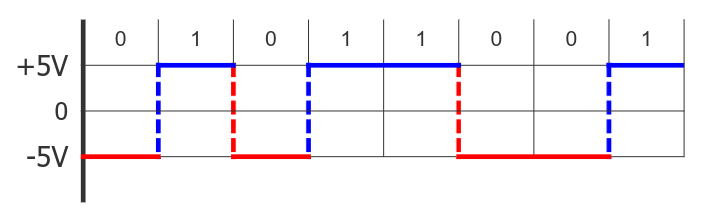
\includegraphics[scale=0.3]{nrz}
\end{center}

\subsubsection{RZ}
Return to zero works on the same principle of NRZ but after each bit the signal goes back to zero first. This way, the signal is \textbf{self-clocking} and there is no direct current. It needs twice the bandwidth.
\begin{center}
	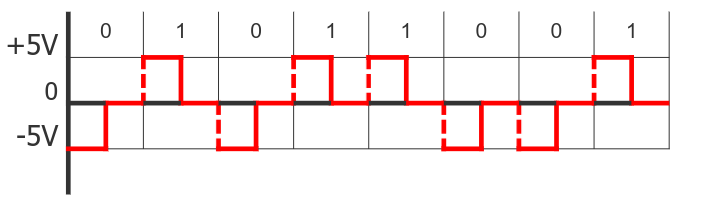
\includegraphics[scale=0.3]{rz}
\end{center}

\subsubsection{Differential NRZ}
Similar principle of NRZ but $1$ is encoded as a \textbf{voltage level change} and $0$ as a missing change, thus having the disadvantages of NRZ only for a sequence of zeros.
\begin{center}
	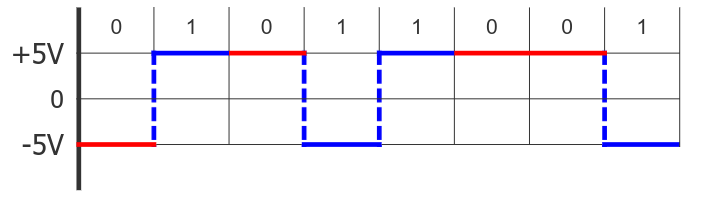
\includegraphics[scale=0.3]{dnrz}
\end{center}

\subsubsection{Manchester code}
With each code element the clock pulse is transferred: voltage level change occurs in the middle of each bit. $0$ is encoded as voltage level change from positive ($+5V$) to negative ($-5V$) while $1$ as voltage level change from negative ($-5V$) to positive ($+5V$).\\
Clock synchronization happens for each bit and the end of the transmission is easily recognizable. The capacity used is only half.
\begin{center}
	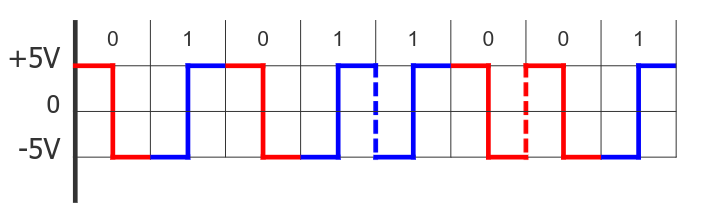
\includegraphics[scale=0.3]{mch}
\end{center}

\subsubsection{Differential Manchester code}
A variant of the Manchester code. $0$ is encoded as a voltage level change while $1$ as a missing one.
\begin{center}
	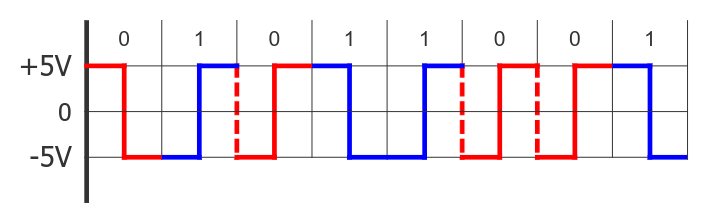
\includegraphics[scale=0.3]{dmch}
\end{center}

\subsubsection{4B/5B}
\begin{wrapfigure}[7]{r}{3.2cm}
	\vspace{-1.5cm}
	\begin{center}
		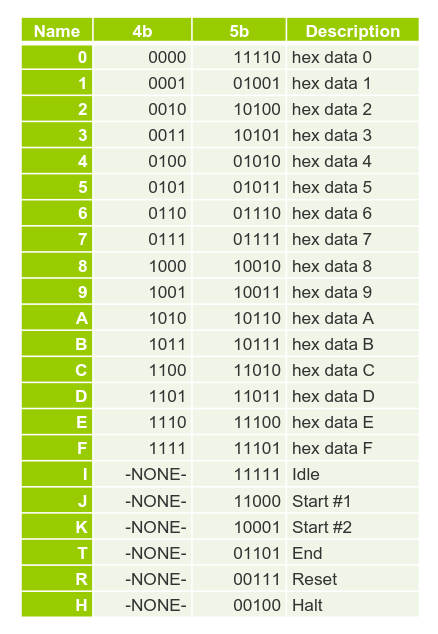
\includegraphics[width=3.2cm]{4b5b}
	\end{center}
\end{wrapfigure}
To improve the efficiency of the Manchester code, this techniques codes a hexadecimal character of four bits in five, avoiding long zero blocks. Uses the same principle of the differential NRZ. Allows some combinations for control information. The transmission provides clocking.\\
It's used in the USB and FastEthernet context and in GigabitEthernet with different variants (8B/10B, 64B/66B, $\ldots$).

\subsection{Modulation}
To transmit with \textbf{broadband} we need to modulate the signal, that being \textbf{shaping} a carrier frequency via the baseband signal.
\begin{equation}
	s(t) = A \cdot \sin(2 \cdot \pi f t + \varphi)
\end{equation}
\subsubsection{ASK}
Modulation of the \textbf{amplitude} $A$. It's easy to realize and doesn't need much bandwidth but it's not robust against distortions. Often used in optical transmissions.
\begin{center}
	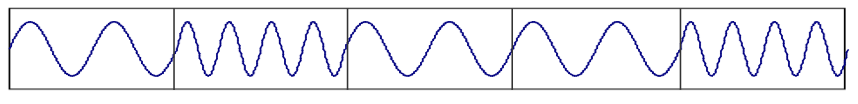
\includegraphics[scale=0.15]{ask}
\end{center}

\subsubsection{FSK}
Modulation of the \textbf{frequency} $f$. It was the first used in data transmission using phone lines. Needs a lot of bandwidth and it's a waste of frequencies.
\begin{center}
	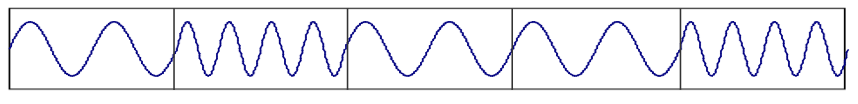
\includegraphics[scale=0.15]{fsk}
\end{center}

\subsubsection{PSK}
Modulation of the \textbf{phase} $\varphi$. It has a complex demodulation process but it's robust against disturbances.
\begin{center}
	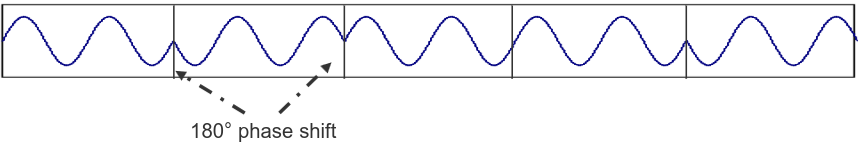
\includegraphics[scale=0.15]{psk}
\end{center}
Also called \textbf{Binary} PSK.

\subsubsection{PSK variants}
\textbf{Quadrature Phase Shifting Key} (also 2B1Q) allows the shifting between $4$ phases, allowing for $4$ states and thus $2$ bits at a time (doubling the data rate).
\begin{center}
	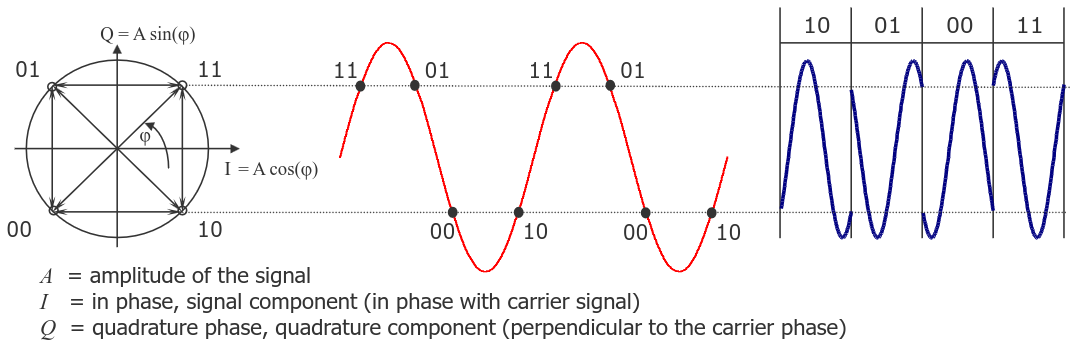
\includegraphics[scale=0.25]{qpsk}
\end{center}
\textbf{Differential} BPSK works with two different phases like PSK but it shifts only if $1$ is the next bit.
\begin{center}
	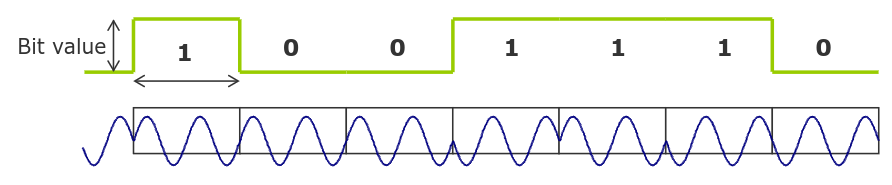
\includegraphics[scale=0.25]{dbpsk}
\end{center}
\textbf{Quadrature Amplitude Modulation} is a combination of ASK and QPSK. $n >2$ bit can be transferred at the same time. Bit error rate increases with $n$ but is still less than similar techniques. Used frequently in wireless communication.
\begin{center}
	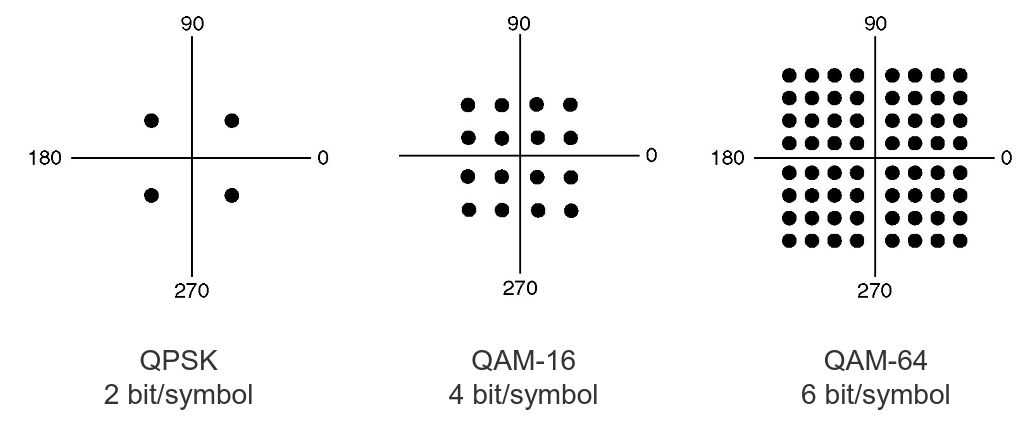
\includegraphics[scale=0.2]{qam}
\end{center}

\subsection{Multiplexing}
Since lines are expensive it's important to share the resources. Multiplexing is a technique that provides simultaneous transmission over a single medium.\\
\begin{wrapfigure}[7]{r}{5cm}
	\begin{center}
		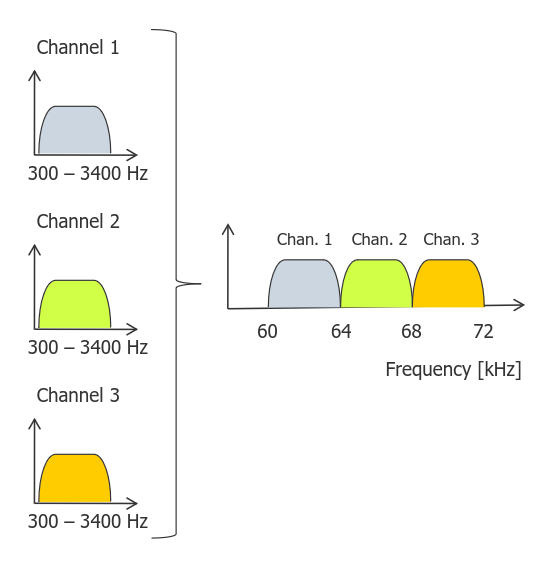
\includegraphics[width=5cm]{fdm}
	\end{center}
\end{wrapfigure}
\subsubsection{FDM}
\textbf{Frequency} Division Multiplexing divides the frequency spectrum in frequency \textbf{bands}, which are used exclusively and simultaneously. When used for optical transmission is called \textbf{Wavelength Division Multiplexing}.
\begin{center}
	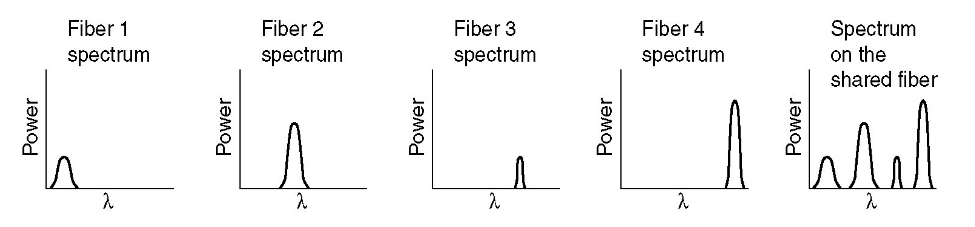
\includegraphics[scale=0.2]{wdm}
\end{center}

\subsubsection{TDM}
\textbf{Time} Division Multiplexing divides time into slots of fixed or variable length. Each timeslot represents one sub-channel.
\begin{center}
	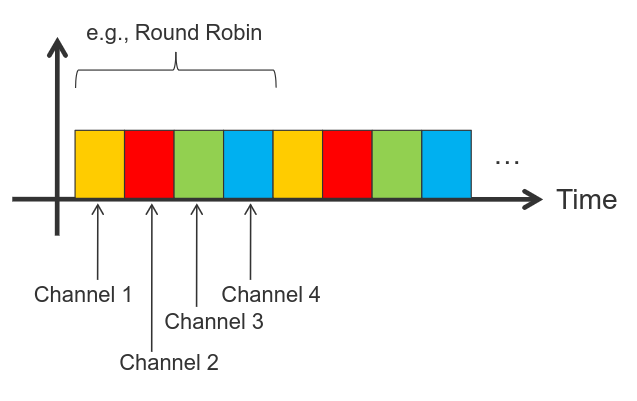
\includegraphics[scale=0.3]{tdm}
\end{center}
A classical TDM is the T1, having $24$ channels in parallel with $8$bit per channel (one is control), a $193$ bit frame that lasts for $125\mu$sec for $1.554$Mbit/s.
\begin{center}
	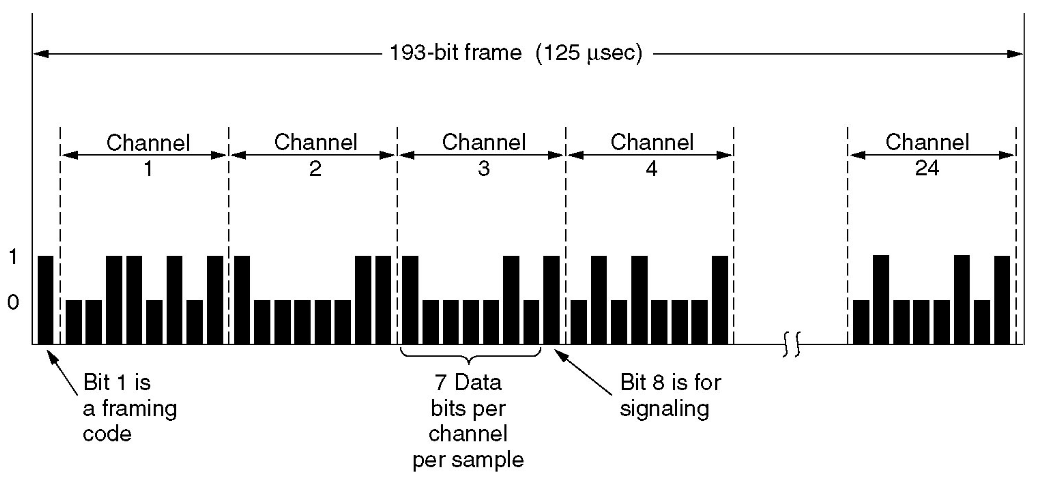
\includegraphics[scale=0.3]{t1}
\end{center}
It's possible to multiplex T1 into higher carriers to get T2, T3, $\ldots$.

\begin{note}
	Multiplexing techniques plus algorithm that control how to do it result in \textbf{Multiple Access} technologies (e.g. FDMA, TDMA) on layer 2.
\end{note}

\newpage
\subsection{Physical media}
There are many different \textbf{medias}.
\begin{center}
	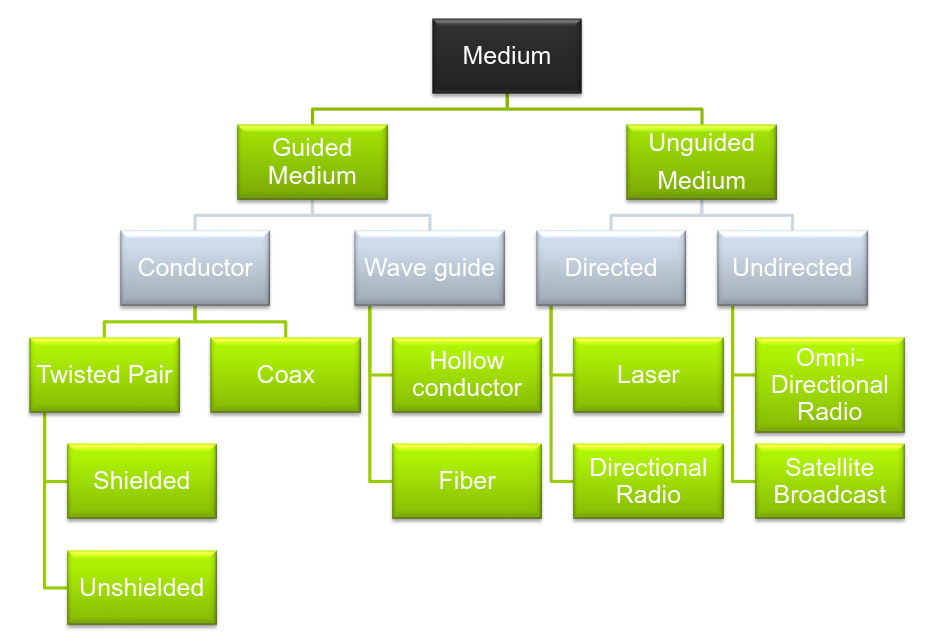
\includegraphics[scale=0.3]{class}
\end{center}
And different type of \textbf{networks}, classified over the size of their scope.
\begin{table}[!h]
	\centering
	\begin{tabular}{|c|c|c|}
		\hline
		\textbf{Name} & \textbf{Scope} & \textbf{Example} \\
		\hline
		\textit{Body/Personal} & 1mt & Body \\
		\hline
		\textit{Local} & 10mt-100mt & Room, Building \\
		\hline
		\textit{Metropolitan} & 1Km-10Km & Campus, Town \\
		\hline
		\textit{Wide} & 100Km-1000Km & Country, Continent \\
		\hline
		\textit{Internet} & 10000Km & Planet \\
		\hline
	\end{tabular}
\end{table}
\subsubsection{Electromagnetic waves}
Electromagnetic waves are used to transmit the signal over cables and wireless. In a vacuum they travel at the speed of light $c$ but in copper or fiber they slow down at about $\frac{2}{3}$ of $c$.\\
The \textbf{fundamental relationship} between wavelength $\lambda$, frequency $f$ and $c$:
\begin{equation}
	\lambda \cdot f = c
\end{equation}

\subsubsection{Guided medium}
\begin{wrapfigure}[7]{r}{3.2cm}
	\vspace{-1cm}
	\begin{center}
		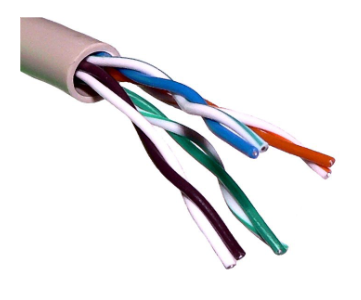
\includegraphics[width=3.2cm]{cable}
	\end{center}
\end{wrapfigure}
\paragraph{Twisted pair} This medium transmits data through \textbf{electrical signals}. Electromagnetic signals from the environment can disturb it, thus it's necessary to have \textbf{insulation} and \textbf{twisting} (also done at different rates to reduce \textbf{crosstalk}). It's cheap and simple and it's used both for digital and analog signals. They have a bit-error rate of $\approx 10^{-5}$.\\
They are divided in:
\begin{itemize}
	\item \textbf{Unshielded} (U)
	\item \textbf{Foil shielded} (F)
	\item \textbf{Screen shielded} (S)
\end{itemize}
The \textbf{shield} can be individual, overall or both. They are also divided in \textbf{categories} based on their shielding level and maximum speed.
\paragraph{Coaxial}
It's a copper cable with braided outer conductor to reduce disturbances and interior insulation between them. Has a bit-rate error of $\approx 10^{-9}$, has higher data rates over longer distances compared to the twisted pair and has a better signal quality.
\begin{center}
	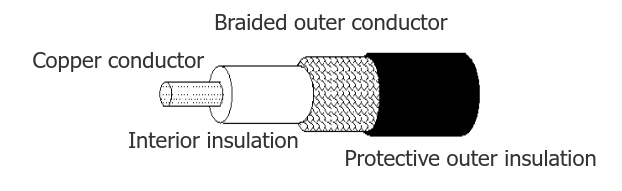
\includegraphics[scale=0.3]{coax}
\end{center}

\paragraph{Optical Fiber}
\begin{wrapfigure}[5]{r}{3.2cm}
	\vspace{-0.5cm}
	\begin{center}
		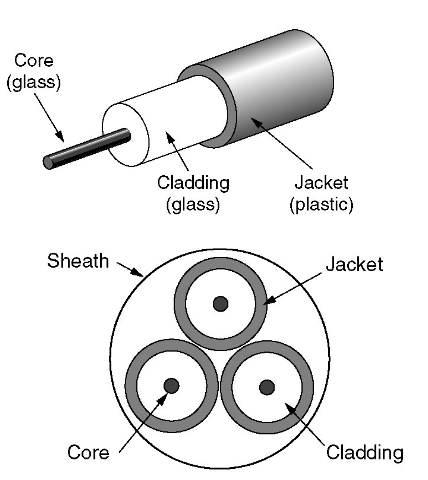
\includegraphics[width=3.2cm]{fibercable}
	\end{center}
\end{wrapfigure}
Huge capacity with nearly unlimited data rate. It's insensitive to electromagnetic disturbances. Has a good signal-to-noise ratio. It's smaller and lighter and has a bit-error rate of $\approx 10^{-12}$.\\
The structure of an optical transmission system has:
\begin{itemize}
	\item \textbf{Light source}: converts electrical into optical signals, $1$ is a light pulse and $0$ is no light pulse
	\item \textbf{Transmission medium}, the optical fiber
	\item \textbf{Detector}: converts optical into electrical signals
\end{itemize}
\begin{center}
	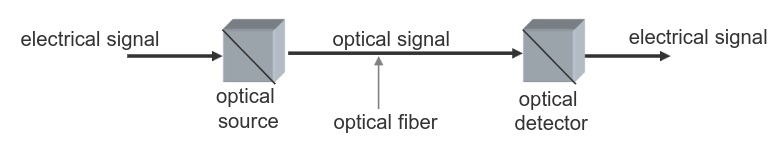
\includegraphics[scale=0.3]{fiber}
\end{center}
The cable has a \textbf{core} made of optical glass (super thin), an internal \textbf{glass cladding} and a protective \textbf{plastic covering}. The transmission takes place in the core, which has a high \textbf{refractive index} (refraction effect relatively to vacuum), where a ray of light is reflected between the two mediums.
\begin{center}
	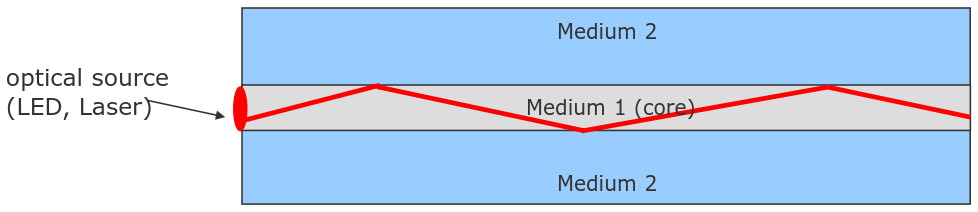
\includegraphics[scale=0.25]{fiberphoto}
\end{center}
There are three types of fiber cables:
\begin{itemize}
	\item \textbf{Single mode}: with a diameter core of $8-10\mu m$, all rays can go in only one direction and therefore having no dispersion (homogeneous signal delay). Expensive due to small core.
	\begin{center}
		\includegraphics[scale=0.3]{single}
	\end{center}
	\item \textbf{Simple multimode} (step index): core diameter of $50\mu m$, uses different wavelengths with different delay signals and therefore has a high dispersion
	\begin{center}
		\includegraphics[scale=0.3]{smulti}
	\end{center}
	\newpage
	\item \textbf{Multimode} with gradient index: same as the simple multimode but the refracting index changes continuously, hence having a low dispersion
	\begin{center}
		\includegraphics[scale=0.3]{multi}
	\end{center}
\end{itemize}

\paragraph{Radiation sources} Radiation sources can be of two types:
\begin{itemize}
	\item \textbf{LED}: cheap and reliable, has a broad wavelength spectrum thus a \textbf{high dispersion} (small range) and a \textbf{low capacity}
	\item \textbf{Laser}: \textbf{expensive} but with \textbf{high capacity} and a small wavelength spectrum and thus \textbf{high range}. They  are sensitive to \textbf{temperatures}.
\end{itemize}
On the other side of the signals there are \textbf{photodiodes}.

\paragraph{Attenuation} The ray of light is increasingly weakened along the medium due to \textbf{absorption} and \textbf{impurities} in it.

\paragraph{Dispersion} Rays of light spread in the medium at different speeds, refractive index in the medium is not constant.

\subsubsection{Home connection}
There are multiple solutions to connect homes to the internet:
\begin{itemize}
	\item Existing \textbf{phone lines} local loop (DSL). It was the first approach. It needed a MoDem (Modulator and Demodulator) to convert digital data into analogs and viceversa. Today uses the whole spectrum of the copper cable and modulates through \textbf{Discrete Multi-Tone} or \textbf{Carrierless Amplitude Phase}. Calls are now over IP. The main standards are VDSL and VDSL2
	\item Existing \textbf{cable TV} network connections, using coaxial and upstream multiplexing through \textbf{Cable Modem Termination System}. Uses the \textbf{DOCSIS} standard.
	\item Deployed \textbf{cellular networks}
	\item Existing \textbf{powerline connections}
	\item \textbf{Satellite} communication
	\item \textbf{Microwave} links
	\item \textbf{Fiber-to-the-home}
\end{itemize}

\paragraph{Discrete Multi-Tone Modulation}
Uses multiple carriers where each channel uses a suitable optimal modulation method (QAM). Channels in high frequencies have a lower quality over long distances.
\begin{center}
	\includegraphics[scale=0.3]{dmt}
\end{center}
% !TeX spellcheck = en_US
\newpage
\section{Link}
\subsection{NIC}
The \textbf{Network Interface Card} is a piece of hardware that provides link layer abstraction to the device network's stack. They are of two types:
\begin{itemize}
	\item \textbf{Point-to-point}: high bandwidth bidirectional links, with a dedicated channel per direction thus avoiding collisions
	\item \textbf{Broadcast}: medium shared in a way that creates collisions if more devices transmit at the same time
\end{itemize}

\subsection{Framing}
Messages are organized in \textbf{frames}, well defined structures, as follows:
\begin{center}
	\includegraphics[scale=0.25]{frame}
\end{center}
\begin{itemize}
	\item \textbf{Preamble}: before the header, flag byte sequence marking the beginning of a frame and sometimes the frame length
	\item \textbf{Header}: control information (e.g. addresses, frame numbers)
	\item \textbf{Error check}: inside the Trailer, contains \textbf{Frame Checking Sequence}
	\item \textbf{Postamble}: after the Trailer, flag byte sequence marking end of a frame
\end{itemize}

\subsubsection{Character count} 
A good addition is using the first value to advertise the number of characters in the frame, thus eliminating the \textit{Postamble}.
\begin{center}
	\includegraphics[scale=0.3]{charcount}
\end{center}

\subsubsection{Character stuffing}
Start and end of a frame are represented by a special byte sequence. Since the flag byte may occur in the payload, \textbf{character} stuffing is done: a special escape byte \textit{ESC} is inserted by the sender and then removed by the receiver. The escape byte may also appear in the payload and thus it may also be stuffed itself.
\begin{center}
	\includegraphics[scale=0.3]{charstuff}
\end{center}
The generic version is the \textbf{bit stuffing}: inserting a $0$ after five consecutive $1$.

\subsubsection{Physical layer}
Framing can also exploit special symbols from the physical layer:
\begin{itemize}
	\item \textbf{4B5B}: use the special symbols as control characters
	\item \textbf{PHY coding violations}: in Manchester code no mid-bit edge can appear, therefore the start and end of a frame can be coded as a violation of that rule
\end{itemize}

\subsection{Error detection and correction}
Transmissions over the physical layer are not error free. Hence, error \textbf{detection} and \textbf{correction }is necessary. The solution is to add \textbf{error control data} to each frame: a frame of $m$ bits receives $r$ check bits, creating a \textbf{codeword} of $n=m+r$ bits.

\subsubsection{Frame Check Sequence}
A very naive solution is to repeat the payload and then do a bit-wise comparison. It's very effective but has a huge \textbf{overhead}.

\paragraph{Parity bit}
This technique reduces the overhead by counting the number of $1$ in the payload and setting the \textbf{parity bit} to $1$ if there is an \textbf{even} amount of them. This adds a $1$bit overhead only but doesn't check for \textit{even} errors and doesn't allow correction.

\paragraph{Double parity}
Group bits together to form a matrix and then compute parity bits for each row and column. Compared to single parity, can identify more errors (not all) and correct some of them.
\begin{center}
	\includegraphics[scale=0.3]{doublepar}
\end{center}

\paragraph{Modulo check}
Parity bits don't handle well error \textbf{bursts\footnote{Group of errors close together, very frequent in data communication.}}. Modulo check tries to solve this by computing a frame check sequence based on a modulo operation: interprets the payload as a number $N$ and appends a control integer $C$ such that
\begin{equation*}
	(N + C) \% 11 = 0
\end{equation*}
Bit errors are detected by recomputing the modulo at the receiver end.
\begin{center}
	\includegraphics[scale=0.3]{modulo}
\end{center}
The generic version is the \textbf{Cyclic Code Checksum}, which allows you to choose the number of bits dedicated to the checksum and the base of the modulo, extremely lowering the probability of undetected errors (if tuned correctly).

\paragraph{Cyclic Redundancy Checksum}
A payload of $m$ bit $a_{m-1}, \ldots, a_0$ is seen as a \textbf{polynomial} $a_{m-1}x^{m-1} + \ldots + a_0$. The sender and the receiver then agree on a \textbf{generator polynomial}
\begin{equation*}
	G(x) = g_r x^r + g_{r-1} x^{r-1} + \ldots + g_1 x^1 + g_0 x^0 \qquad\qquad g_r = g_0 = 1
\end{equation*}
The sender then interprets a data block of length $m$ as a polynomial 
\begin{equation*}
	M(x) = a_{m-1}x^{m-1} + \ldots + a_1x^1 + a_0x^0
\end{equation*}
and adds redundant bits so that the extended polynomial $M'(x)$ is divisible by $G(x)$.
\begin{lstlisting}[mathescape=true]
	r = degree(generator_polynomial)
	extended_data_bits = data_bits + (r zeros)  // Concatenate r zeros
	remainder_bits = binary_division(extended_data_bits, generator_polynomial)
	checksummed_frame = extended_data_bits XOR remainder_bits
\end{lstlisting}
On the other hand the receiver divides the received extended polynomial $M'(x)$ by $G(x)$ and if the remainder is $0$ then no error occurred.\\
CRC will detect all error bursts of length $\leq r$. It \textbf{will not recognize} if instead of $T(x)$, $T(x)+E(x)$ with $E(x)$ containing $G(x)$ as a factor.
\begin{note}
	Common 16-bit generators are:
	\begin{itemize}
		\item \textbf{CRC-16} $G(x) = x^{16} + x^{15} + x^2 +1$
		\item \textbf{CRC CITT} $G(x) = x^{16} + x^{12} + x^5 + 1$
		\item \textbf{Ethernet} $G(x) = x^32 + x^{26} + x^{23} + x^{22} + x^{16} + x^{12} + x^{11} + x^{10} + x^8 + x^7 + x^5 + x^4 +x^2 + x+1$
	\end{itemize}
\end{note}
The \textbf{hardware} implementation for CRC uses \textbf{shift registers} with XOR for subtraction and AND for applying it.
\begin{example}
	Circuit for the generator polynomial
	\begin{equation*}
		G(x) = x^4 + x + 1
	\end{equation*}
	\begin{center}
		\includegraphics[scale=0.4]{crc}
	\end{center}
\end{example}

\subsubsection{Hamming Distance}
The Hamming Distance is the number of places in which two binary sequences differ. Given an $m$bit long \textbf{data} with $2^m$ possible \textit{data words}, $r$ \textbf{check bits} and thus $n=m+r$ bit \textbf{codewords}, build a list of all the possible $2^n$ codewords and find the two with the minimum distance. This allows to:
\begin{itemize}
	\item \textbf{Detect} $d$ errors, having a distance of at least $d+1$
	\item \textbf{Correct} $d$ errors, having a distance of at least $2d+1$
\end{itemize}

\begin{example}
	Given a code with only two possible codewords:
	\begin{align*}
		& w_1=000 \\
		& w_2 = 111
	\end{align*}
	We have a distance of $3$, meaning we can \textbf{detect} $2$ bits errors and correct $1$bit ones:
	\begin{itemize}
		\item $001$ received, we can correct it
		\item $110$ received, cannot be recovered
	\end{itemize}
\end{example}

While the Hamming Code can correctly identify and correct $1$bit errors, it's expensive in terms of required check bits and can't correct $2$bits errors and cannot identify $3$bits ones.

\subsubsection{Correction mechanism}
\paragraph{Forward Error Correction} Uses error correcting codes (RS, BCH): they can be corrected in most cases, \textbf{discarded} otherwise. It's low latency since the feedback from the receiver to the sender is not needed, therefore suitable for \textbf{delay sensitive} transmissions.

\paragraph{Automatic Repeat reQuest}
Uses error-detecting codes (CRC): if data contains errors, it needs to be sent again from the sender. Suitable for \textbf{error sensitive} transmissions. Using ARQ means managing the \textbf{control flow} (numbering data blocks, receipt acknowledgment, retransmission).

\subsection{Flow control}
Let's define a sketch of the interface between the Link layer and the Network and Physical layers.
\begin{lstlisting}[language=C]
	#define MAX_PKT 1024 /* determines packet size in bytes */
	
	typedef enum {false, true} boolean; /* boolean type */
	
	typedef unsigned int seq_nr; /* sequence or ack numbers */
	
	typedef struct {
		unsigned char data[MAX_PKT];
	} packet; /* packet definition */
	
	typedef enum {data, ack, nak} frame_kind; /* kinds of frames */
	
	typedef struct { /* frames are transported in this layer */
		frame_type type; /* what kind of a frame is it? */
		seq_nr seq; /* sequence number */
		seq_nr ack; /* acknowledgement number */
		packet info; /* the network layer packet */
	} frame;
\end{lstlisting}
\begin{center}
	\includegraphics[scale=0.27]{interface}
\end{center}

\subsubsection{Simplex}
\begin{wrapfigure}[14]{r}{7cm}
	\begin{center}
		\includegraphics[width=7cm]{simplex}
	\end{center}
\end{wrapfigure}
This is the simplest mechanism of flow control: transmission happens in \textbf{one direction} without \textit{sequence number} or \textit{acknowledgment} and ignoring \textit{processing time}. The sender \textbf{fetches} and \textbf{sends} data in an infinite loop, while the receiver \textbf{gets} it and \textbf{forwards} it to the network layer.
While being extremely \textbf{simple}, it assumes that the channel never damages or loses frames and that the \textbf{network layer} is \textbf{always ready}.\\\\
To solve all of these problems we have two approaches:
\begin{itemize}
	\item \textbf{Feedback} based flow control: receiver sends information back to the sender allowing him to send more data
	\item \textbf{Rate} based flow control: protocols limits the data a sender may transmit without feedback from the receiver
\end{itemize}

\subsubsection{Stop-and-wait}
\begin{wrapfigure}[14]{r}{7cm}
	\vspace{-1cm}
	\begin{center}
		\includegraphics[width=7cm]{stopwait}
	\end{center}
\end{wrapfigure}
This approach uses a \textbf{bidirectional channel}: the sender sends a data blocks and waits until an \textbf{acknowledgment} from the receiver arrives or a \textbf{timeout} is reached. An unacknowledged data block is resent.\\\\
Since the channel is not error-free, we use the \textbf{Alternating Bit Protocol} to signal a duplicate data block by using one bit flag.\\\\
The main drawback is that there are large waiting periods between the transmissions, hence \textbf{capacity is wasted}.

\paragraph{Piggybacking}
To get a \textbf{full-duplex} communication we could use two simplex channels with \textbf{stop-and-wait}. That would be a waste of resource, hence the technique of \textbf{piggybacking}.\\
It consists of \textbf{stop-and-wait} on a single channel for both directions: data frames and ACK are intermixed and distinguished by the \textbf{Type} field in the header.\\
An even more efficient approach is to include the ACK message in header of the data frame. When a data packet arrives, the receiver waits a particular time interval to send the ACK back.

\begin{figure}[!h]
	\hfil
	\subfigure[Separate messages]{\includegraphics[scale=0.4]{ack1}}
	\hfil
	\subfigure[Single message]{\includegraphics[scale=0.4]{ack2}}
\end{figure}

\subsubsection{Sliding window}
To avoid long waiting periods of the sender, both parts agree on a \textbf{transmission window} of size $W$. Any message sent in that window doesn't need a specific ACK, when ACK is sent all previous messages in the window are acknowledged.\\
For this technique, \textbf{sequence numbers} need to be introduced, to allow sequentially numbering of the messages. If coded on $n$bits, the sequence number $\text{seqnum} \in \{0, 1, \ldots, 2^n-1\}$ and \textbf{wraps around} the end.

\begin{note}
	All frames in the window must be \textbf{buffered}, hence for a window of size $W$ a buffer for $W$ frames is needed.
\end{note}

\begin{observation}
	It's important to have a window of size $W < 2^n$ and not $W \leq 2^n$ to avoid ambiguities.
\end{observation}

\paragraph{Pipelining}
Long round-trip time is an issue in terms of efficiency. If $\text{bandwidth} \cdot \text{round-trip-delay}$ is large, a big window is needed to fill the pipe capacity. Having a bigger window size means also having more bit-errors and packet loss.\newpage
\noindent There are three ways of handling the \textbf{pipelining}:
\begin{itemize}
	\item \textbf{Go-back-N}: each frame has an associated \textbf{timer} of the expected time to receive an ACK. When an ACK is received a new packet is sent and the buffer is updated (window slide). When the timer expires, the sender retransmits all buffered frames.
	\item \textbf{Selective repeat}: when a frame is correct, send ACK. When it's missing, \textbf{buffer} the following correct frames. When the missing message arrives, send ACK for that one and all the buffered frames. Capacity is used more efficiently but the receiver needs more buffer.
	\item \textbf{Selective reject}: works similar to selective repeat but when a frame is missing, a negative acknowledgment is sent and just that frame is repeated. A variation is to send a list of missing frames instead of a single NACK. This method enhances \textbf{efficiency} but it's more complex.
\end{itemize}

\begin{figure}[!h]
	\hfil
	\subfigure[Go-back-N]{\includegraphics[scale=0.3]{gobackn}}
	\hfil
	\subfigure[Selective repeat]{\includegraphics[scale=0.3]{srep}}
	\hfil
	\subfigure[Selective reject]{\includegraphics[scale=0.3]{srej}}
\end{figure}

\begin{note}
	Some protocols require many timers: implement them by using one hardware timer and store expiration times in a linked list that's updated during protocol runtime.
	\begin{center}
		\includegraphics[scale=0.4]{timer}
	\end{center}
\end{note}

\newpage
\subsection{Medium Access Control}
When dealing with a medium shared by $n>2$ nodes, a NIC needs to manage:
\begin{itemize}
	\item \textbf{Channel allocation}: medium access control, organizes the order of transmitting nodes on the channel. There are two different approaches:
	\begin{itemize}
		\item \textbf{Distributed MAC}: there are $n$ nodes that generate frames for transmission on shared single channel. If two frames are transmitted simultaneously, the frames are lost. Time management can happen in two ways:
		\begin{itemize}
			\item \textbf{Continuous} time: no master clock, transmission of frames can begin at any time
			\item \textbf{Slotted} time: time is divided into discrete intervals (slot), frame transmission begins always at the start of a slot
		\end{itemize}
		\item \textbf{Centralized MAC}: a \textbf{master device} manages channel allocation
		\begin{itemize}
			\item \textbf{Round-Robin}: the master device polls each node periodically (fixed TDMA) and each node gets the entire transmission capacity for a fixed time interval
			\begin{center}
				\includegraphics[scale=0.3]{ftdma}
			\end{center}
			\item \textbf{FDMA}: the master allocates a different frequency to each node, which gets a portion of the transmission capacity for the whole time
			\begin{center}
				\includegraphics[scale=0.3]{fdma}
			\end{center}
		\end{itemize}
		Since users are typically \textbf{bursty}, most subchannels will be idle most of the time.
	\end{itemize}
	\item \textbf{Node identification}: addresses of the nodes on the medium, \textbf{MAC Addresses}, typically $6$bytes long in hexadecimal notation
\end{itemize}

\subsubsection{Token}
\begin{wrapfigure}[5]{r}{3cm}
	\vspace{-1.5cm}
	\begin{center}
		\includegraphics[width=3cm]{token}
	\end{center}
\end{wrapfigure}
Multiple access using a \textbf{token} (a bit sequence) means that only the owner of the token is allowed to send. The token is then passed between all the nodes. It's particularly suitable for a \textbf{ring} topology. It guarantees access without collisions, efficient and fair. It's very complex, e.g. when handling a lost token.

\subsubsection{ALOHA}
This multiple access technique was derived from the principles of \textit{ALOHANET}\footnote{Developed by Norman Abramson on the Hawaiian Islands in 1970s, a network connecting computers on islands over radio. There were two channels: uplink shared by nodes (collision may occur) and downlink used by main computer. The packets were ACKed by the main computer. Good performance only in low traffic.}. Nodes are \textbf{uncoordinated} and they can send at any time on every frequency. When several nodes are sending at the same time, a \textbf{collision} occurs: the frame are lost and each sender wait a \textbf{random time} to transmit again.

\begin{center}
	\includegraphics[scale=0.4]{aloha}
\end{center}

\paragraph{Slotted ALOHA} Even small overlaps would cause a collision, hence having a \textbf{low throughput} and no guaranteed response time. The improvement was \textbf{slotted} ALOHA: the time axis was divided into \textbf{time slots} and each sender could send at any time but only at the beginning of a time slot. This brought fewer collisions but now \textbf{synchronization} of the computers was needed.

\begin{center}
	\includegraphics[scale=0.4]{slotaloha}
\end{center}

\paragraph{Performance}
Given an infinite number of users generating data, the transmissions (and retransmissions) are generated according to a Poisson distribution with intensity $\lambda$. Hence, the probability of $k$ transmission attempts in an interval $[0,t)$ is
\begin{equation*}
	P(X=k)=\frac{(\lambda t)^k}{k!}\cdot e^{-\lambda t}
\end{equation*}
The \textbf{throughput} $S$ is given by the load $G$ and the probability of a \textbf{successful} transmission $P_0$
\begin{equation*}
	S=G \cdot P_0
\end{equation*}
A frame is \textbf{successfully} transmitted if no other frames are within the \textbf{vulnerability period} $t$
\begin{equation*}
	P_0 = P(X=0)=\frac{(Gt)^0}{0!}\cdot e^{-Gt} = e^{-Gt}
\end{equation*}
Then, assuming that time unit is the time to send a single frame, we have:
\begin{itemize}
	\item \textbf{ALOHA} with vulnerability period of $2$
	\begin{equation*}
		S=G\cdot P_0 = G \cdot e^{-2G}
	\end{equation*}
	\item \textbf{Slotted ALOHA} with vulnerability period of $1$
	\begin{equation*}
		S=G\cdot P_0 = G \cdot e^{-G}
	\end{equation*}
\end{itemize}
\begin{center}
	\includegraphics[scale=0.3]{alohaper}
\end{center}

\newpage
\subsubsection{CSMA}
Since ALOHA doesn't perform well under high loads, a solution is to reduce collisions: a sender first examines if another node is already transmitting and if nobody is currently sending, they are free to start. This is called \textbf{Carrier Sense Multiple Access} and it's a \textbf{simple} way with good utilization of the network. The main drawback is that there is \textbf{no guarantee} for the access to the medium. It only works with \textbf{short transmission delay}.\\
There are three variants:
\begin{itemize}
	\item \textbf{Non persistent}: when a node has data to send, it first listens to the channel. If it's busy, the computer listens and waits for availability. As soon as the channel is idle, the frame is transmitted. If a collision occurs, the node waits a random amount of time and starts again.
	\item \textbf{Persistent}: when a node has data to send, it first listens to the channel. If it's busy, the node waits a random amount of time and starts again. Else, it starts transmitting.
	\item $p$\textbf{-persistent}: if the channel is idle, a node that has data to send transmits with \textbf{probability} $p$ in current slot and defers until next slot with probability $(1-p)$ going then back to the beginning. If the channel is busy, the node waits from the next slot and goes back to the beginning. If a collision occurs, the node waits a random amount of time and goes back to the beginning. It's applicable in slotted time environments (slotted ALOHA).
\end{itemize}

\begin{center}
	\includegraphics[scale=0.3]{csma}
\end{center}

\paragraph{CSMA/CD}
CSMA with \textbf{Collision Detection} aims to reduce the waste produced by collisions between long frames: the node listens through their own transmission, if what they hear is different from what they sent, stop the transmission and wait a random amount of time.
\begin{center}
	\includegraphics[scale=.3]{csmacd}
\end{center}

\subsubsection{Reservation mechanisms}
Reserve the channel to avoid collisions. Works in two \textbf{alternating phases}:
\begin{enumerate}
	\item \textbf{Reservation}: the sender makes a reservation by indicating the wish to send data (in some cases also the length)
	\item \textbf{Transmission}: if reservation is ok, the data communication takes place 
\end{enumerate}
It's very efficient in terms of capacity but there is more delay due to the reservation procedure.\\
The reservation can be:
\begin{itemize}
	\item \textbf{Centralized}: a master periodically queries all the nodes and checks if they have to send data, assigning sending rights
	\item \textbf{Distributed}
	\begin{itemize}
		\item \textit{Explicit}: \textbf{Bit-Map} approach, uses a small \textbf{reservation frame} in the first phase and a \textbf{data frame} of constant size in the second phase. There are two variants:
		\begin{itemize}
			\item \textbf{Without contention}: each user $i$ is assigned to the $i$th slot in the reservation frame. If it wants to send the data, it sets the bit to $1$. After the reservation phase, all nodes have set their bit and can send the data in the order of the bits in the frame
			\begin{center}
				\includegraphics[scale=.3]{bitmap1}
			\end{center}
			\item \textbf{With contention}: the reservation frame consists of a limited number of contention slots  $<i$. Users try to get a random contention slot writing their computer ID into a slot. If there is no collision in the reservation phase, a node may send.
			\begin{center}
				\includegraphics[scale=.3]{bitmap2}
			\end{center}
		\end{itemize}
		\item \textit{Implicit}
		\begin{itemize}
			\item \textbf{Binary Countdown}: there are priorities based on the ID of the computer. When nodes need to send data, they enter a \textbf{contention} phase where they broadcast their ID bit by bit. The smaller addresses give up.
			\item \textbf{Adaptive Tree Walk}: the nodes are the leaves of a binary tree. In the first contention slot following a successful frame (slot $0$), all nodes are allowed to try to acquire the channel. If there is a collision, only the nodes from the left subtree are allowed to try. If successful, the slot is reserved for the right subtree.
		\end{itemize}
	\end{itemize}
\end{itemize}

\subsection{Protocols}
\subsubsection{PPP}
\textbf{Point to Point Protocol} establishes a direct connection between two nodes. It supports synchronous and asynchronous connections. It uses:
\begin{itemize}
	\item Specified \textbf{frame format} with \textbf{error detection}
	\item \textbf{Sliding window} approach for flow control
	\item Specified connection establishment and tear down
\end{itemize}
It doesn't use medium access control since there is no need to on point-to-point links.
\paragraph{Connection} The connection happens in three steps:
\begin{enumerate}
	\item PPP establishes a \textbf{basic physical layer connection}, testing that the layer is ready
	\item \textbf{Link Control Protocol} configures the NIC on each end of the link:
	\begin{itemize}
		\item \textit{Maximum Frame Size} (MTU)
		\item \textit{Escape characters}
		\item \textit{Magic numbers}: identifying an end or to detect looped links
		\item \textit{Authentication method}
	\end{itemize}
	It also manages the \textbf{termination} of the link layer connection.
	\newpage
	The \textbf{frame types} are defined between the \textit{initiator} and the \textit{responder} as follows:
	\begin{table}[!h]
		\centering
		\begin{tabular}{|c|c|c|}
			\hline
			\textbf{Name} & \textbf{Direction} & \textbf{Description}\\
			\hline
			\textit{configure-request} & $I \to R$ & List of proposed options and values \\
			\hline
			\textit{configure-ack} & $I \leftarrow R$ & All options are accepted \\
			\hline
			\textit{configure-nack}& $I \leftarrow R$ & Some options are not accepted \\
			\hline
			\textit{configure-reject} & $I \leftarrow R$ & Some options are non negotiable \\
			\hline
			\textit{terminate-request} & $I \to R$ & Request to shut the line down \\
			\hline
			\textit{terminate-ack} & $I \leftarrow R$ & OK, line shutdown \\
			\hline
			\textit{code-reject} & $I \leftarrow R$ & Unknown request received \\
			\hline
			\textit{protocol-reject} & $I \leftarrow R$ & Unknown protocol requested \\
			\hline
			\textit{echo-request} & $I \to R$ & Send this frame back \\
			\hline
			\textit{echo-reply} & $I \leftarrow R$ & Here is the frame back \\
			\hline
			\textit{discard-request} & $I \to R$ & Just discard this frame (testing)\\
			\hline
		\end{tabular}
	\end{table}
	\item \textbf{Network Control Protocol} negotiates the network layer conditions (e.g. Internet Protocol Control Protocol configures IPv4 networks address or compression options) and manages the tear down of the network layer connection (frees IP)
\end{enumerate}

\begin{center}
	\includegraphics[scale=.25]{pppstates}
\end{center}
PPP is \textbf{character oriented} (byte oriented) and uses \textbf{byte stuffing}.
\begin{center}
	\includegraphics[scale=0.4]{ppp}
\end{center}
\begin{itemize}
	\item \textbf{Flag}: start of frame with special flag $01111110$ while end of frame is omitted for successive frames
	\item \textbf{Address}: useless, inherited from HDLC, it's set to $11111111$
	\item \textbf{Control}: set to \textbf{unnumbered mode} $00000011$, meaning without sequence numbering and acknowledgments
	\item \textbf{Protocol}: specifies to which network layer the payload should be delivered. For IP it's $00000110$
	\item \textbf{Checksum}: just \textbf{detection}, default is $16$ bit CRC with generator polynomial $x^{16}+x^{12}+x^5+1$ computed over \textit{Address}, \textit{Control}, \textit{Protocol}, \textit{Payload} and \textit{Padding}
\end{itemize}

\paragraph{Usage} PPP used to be the default link layer protocol for \textbf{dial-up} internet access. Now it's still used on \textbf{point-to-point optical links} (PPPoE) and for the last mile with DSL (PPPoA).

\subsubsection{Ethernet}
\paragraph{History} After ALOHA, Xerox began experimentation on network over \textbf{coaxial} cables. In 1976 Robert Metcalf created Ethernet, an improvement over ALOHA  with CSMA/CD. Between 1978 and 1983 the new standard IEEE 802.3 was created.\\
Initially it was a network over a \textbf{bus} topology: it was hard to maintain and debug if the bus got damaged. The solution was to implement a \textbf{star} topology where the cable goes through a central point: initially a \textbf{hub} (just a repeater, still CSMA/CD) and later a \textbf{switch} (one NIC per interface, no need of CSMA/CD).

\paragraph{Frame}
\begin{center}
	\includegraphics[scale=.3]{ethframe}
\end{center}
\begin{itemize}
	\item \textbf{Preamble}: 7 bytes, each one $10101010$, flag for synchronization
	\item \textbf{Start Frame Delimiter}: one byte $10101011$ marking the beginning of the frame
	\item \textbf{Destination address}: $6$ bytes containing the MAC address of the receiver
	\item \textbf{Source Address}: $6$ bytes containing the MAC address of the sender
	\item Depending on the version
	\begin{itemize}
		\item \textbf{Data length} in 802.3, ranging from $0$ to $1500$
		\item Identification of the \textbf{upper layer protocol} in Ethernet II
	\end{itemize}
	\item \textbf{Data}
	\item From $0$ to $46$ bytes of \textbf{padding} to fill up the frame to at least $64$ bytes, otherwise small fragments are discarded
	\item \textbf{Frame Check Sequence}: $4$ bytes that uses a $32$bit CRC computed over \textit{DA}, \textit{SA}, \textit{length}/\textit{type},\textit{data} and \textit{padding}
\end{itemize}

\paragraph{MAC Address}
\begin{wrapfigure}[5]{r}{6cm}
	\vspace{-.5cm}
	\begin{center}
		\includegraphics[width=6cm]{mac}
	\end{center}
\end{wrapfigure}
The MAC address is a $6$ bytes long number assigned uniquely by IEEE and locally administered. It can be:
\begin{itemize}
	\item \textbf{Unicast}, starting with $0$
	\item \textbf{Multicast}, starting with $1$
	\item \textbf{Broadcast} with all $1$
\end{itemize}

\paragraph{Multiple Access Control} Ethernet collision resolution mechanism is based on CSMA/CD: listen before sending and stop as soon as simultaneous transmissions are detected. A simple solution but with a possible large delay before sending.\\\\
The waiting period after a collision needs to be kept small to avoid long delays but at the same time that makes the risk of subsequent conflict higher. The solution is \textbf{Binary Exponential Backoff}: the random waiting period is drawn from an \textbf{increasing interval}. After $i$ collisions the node waits drawing a random number between $[0, 2^i-1]$, after $10$ collisions the interval becomes $0, 2^{10}-1$ and after $16$ the node gives up.\\\\
When the channel is free again the node waits $x$ time slots before starting again, where a \textbf{time slot} corresponds to the minimum Ethernet frame length.\\\\
The major drawback is that it tends to prefer last contention winners and new contending nodes over the others, being \textbf{unfair}.

\begin{observation}[Collision detection]
	Since the propagation speed is \textbf{finite}, collision detection is not instantaneous. The solution is to adjust \textbf{minimum packet length} and \textbf{maximum traveled distance}. A node needs to be sure that the beginning of its message reached the receiver before assuming there  was no collision and stops listening.
\end{observation}

\paragraph{Physical layer} The physical layer used with Ethernet is \textbf{baseband} encoding with \textbf{Manchester Encoding}. The voltages used are $\pm 0.85V$.

\paragraph{Standards} Some Ethernet standards are:
\begin{itemize}
	\item \textbf{10Base-2} (cheapnet): cheap coaxial cable. Terminals are attached with BNC connectors, maximum $5$ segments, $30$ nodes per segment, at least $0.5m$ between each node, $185m$ maximum segment length and a maximum expansion of $925m$
	\item \textbf{10Base-T} (twisted pair): star topology using twisted pair where several nodes are connected through a hub. Devices are attached with a RJ45 plug where 2 out of 4 cables are used. Maximum cable length to the hub is $100m$ and maximum extension $200m$
	\item \textbf{10Base-F}: Ethernet with fiber optics, expensive but excellent against noise. Used to connect distant buildings
	\item \textbf{Fast Ethernet}: concept based on \textit{10Base-T} with a central hub or switch. $100$Mbps transmission rate. The speed was a problem for the collision detection, hence the maximum distance was reduced to $200$m. It also brought \textbf{auto-configuration} of NICs (speed and communication mode)
	\begin{itemize}
		\item \textbf{100Base-T4}: UTP cable CAT3, using all the 4 cables pairs, and 8B6T encoding
		\item \textbf{100Base-TX}: UTP cable CAT5, using only 2 cable pairs, and 4B5B encoding
		\item \textbf{100Base-FX}: optical fiber, one per direction, with a maximum cable length to the hub of $400$m. There is a variant where only switches are allowed and the maximum length is $2$Km
	\end{itemize}
	\item \textbf{Gigabit Ethernet}: to avoid reducing the cable length while maintaining a high speed, a new minimum frame length of $512$ bytes was specified. The \textbf{Carrier Extension} was made through a \textit{nodata} field after the FCS. This field is added by the hardware while the software is kept unaware.
	\begin{center}
		\includegraphics[scale=.2]{giga}
	\end{center}
	Now the sending of several successive frames (\textbf{Frame Bursts}) is possible without the need of repeated CSMA/CD: the sending MAC fills the gaps between the frames with \textbf{Interframe-Bits} (IFG), signaling to other nodes that the medium is still occupied.
	\begin{center}
		\includegraphics[scale=.2]{giga2}
	\end{center}
	\begin{itemize}
		\item \textbf{1000Base-T}: UTP cable CAT5/6/7, uses 4 pairs, maximum segment length of $100$m
		\item \textbf{1000Base-CX}: STP cable, uses 2 pairs, maximum segment length of $25$m
		\item \textbf{1000Base-SX}: multimode fiber with a maximum length of $550$m and on the $850$nm band
		\item \textbf{1000Base-LX}: single or multimode fiber over $5000$m and on $1300$nm band
	\end{itemize}
	\item \textbf{10-Gigabit Ethernet}: star topology using switch and optical fibers. CSMA/CD is no longer used since collisions cannot occur. There are two specifications on the physical layer:
	\begin{itemize}
		\item \textbf{LAN} with $10$Gbps
		\item \textbf{WAN} with $9.6215$Gbps for compatibility with SDH/SONET
	\end{itemize}
	The \textbf{copper} variants are:
	\begin{itemize}
		\item \textbf{10GBase-CX4}: four pairs of coaxial cables for each direction, maximum length of $15$m
		\item \textbf{10GBase-T}: either CAT6 ($50$m) or CAT7 ($100m$) cables, uses all the pairs in both directions in parallel, there is a filter for each cable to separate the sending and the receiving. On the physical layer a variant of \textbf{Pulse Amplitude Modulation} is used, with $16$ discrete levels between $\pm 1V$
	\end{itemize}
	The \textbf{fiber} variants are:
	\begin{table}[!h]
		\centering
		\begin{tabular}{|c|c|c|c|c|c|c|}
			\hline
			\textbf{Name} & \textbf{Type} & \textbf{Wavelength (nm)} & \textbf{PHY} & \textbf{Coding} & \textbf{Fiber} & \textbf{Range(m)} \\
			\hline
			\textit{10Base-SR} & Serial\footnotemark& $850$ & LAN & 64B66B & Multimode & $26-400$\\
			\hline
			\textit{10Base-LR} & Serial & $310$ & LAN & 64B66B & Singlemode & $10.000$\\
			\hline
			\textit{10Base-ER} & Serial & $1550$ & LAN & 64B66B & Singlemode & $40.000$\\
			\hline
			\textit{10Base-LX4} & WDM\footnotemark& $1275, 1300, 1325, 1350$ & LAN & 8B10B & Both & $10.000$\\
			\hline
			\textit{10Base-SW} & Serial & $850$ & WAN & 64B66B & Multimode & $26-65$\\
			\hline
			\textit{10Base-LW} & Serial & $1310$ & WAN& 64B66B & Singlemode & $10.000$\\
			\hline
			\textit{10Base-EW} & Serial & $1550$ & WAN& 64B66B & Singlemode & $40.000$\\
			\hline
		\end{tabular}
	\end{table}
\end{itemize}
\footnotetext{Only one transmission at a time.}
\footnotetext{Wavelength Division Multiplexing: several transmissions in parallel.} 

\paragraph{Logical Link Control} LLC interfaces with the network layer to provide:\\
\begin{wrapfigure}[5]{r}{5cm}
	\begin{center}
		\includegraphics[width=5cm]{llc}
	\end{center}
\end{wrapfigure}
\begin{itemize}
	\item \textbf{Unreliable} datagram service
	\item \textbf{Acknowledged} datagram service
	\item \textbf{Reliable connection-oriented} service
\end{itemize}
The header contains:
\begin{itemize}
	\item \textbf{Destination} access point: which process to deliver
	\item \textbf{Source} access point
	\item \textbf{Control} field for sequence and ack numbers
\end{itemize}
Today it's \textbf{disbanded}.

\subsection{Infrastructure}
Different devices are used in different layers of a network.
\begin{center}
	\includegraphics[scale=0.4]{infrastructure}
\end{center}

\newpage
\subsubsection{Physical elements}
\paragraph{Hub and Repeaters} A \textbf{Hub} sends the received packets on one side to all of the devices on the other side. A \textbf{repeater} links two different networks. Both of them do not understand packets, frames or headers: they just refresh the signal and \textbf{increase} the network \textbf{range}. They offer one channel shared between all nodes, a low cost but also low security solution.
\begin{figure}[!h]
	\hfil
	\subfigure[Hub]{\includegraphics[scale=0.3]{hub}}
	\hfil
	\subfigure[Repeater]{\includegraphics[scale=0.3]{repeater}}
\end{figure}

\paragraph{Bridging} Since many LAN exists due to load management reasons, security reasons and maximum length reasons, it's fundamental to connect them. A bridge should be \textbf{transparent} (different formats, data rates, lengths) and \textbf{flexible} (moving a node between networks should not require new HW or SW).\\
A bridge operates at the link layer, it processes frame addresses and supports different network types.

\begin{center}
	\includegraphics[scale=.3]{bridge}
\end{center}

\noindent Each bridge has a \textbf{forwarding database} with at least two entries. Each entry has:
\begin{itemize}
	\item \textbf{MAC Address}: host ID
	\item \textbf{Port}: port number of the bridge used to send data to the host
	\item \textbf{Age}: aging time of entry (optional)
\end{itemize}
The source field of a frame that arrives on a port tells which hosts are reachable from this port. For each frame received the bridge stores the source field in the database together with the port where the frame was received. All entries are deleted after a certain amount of time.

\subparagraph{Spanning Tree Protocol} Adding redundancy in a network will introduce \textbf{endless loops}. The idea behind a Spanning Tree is to relay frames only along the edges of a tree structure. It works as follows:
\begin{itemize}
	\item At the beginning each bridge assumes to be root and floods a packet containing its ID and current cost initialized at $0$ over all of its ports
	\begin{center}
		\includegraphics[scale=.3]{stp}
	\end{center}
	\item A bridge that receives such packet checks the root ID and compares it with its own. Both the ID and the costs are updated (its own cost for the sender bridge is summed with current cost value) for receiving packets with smaller ID and forwarded
	\item When the updated packets of all bridges have passed all other, there is an agreement on the \textbf{root bridge}. The received packets containing the smallest costs determine the \textbf{designated bridge} for a LAN and designated ports for the bridges to send out data
\end{itemize}

\paragraph{Switches}
\begin{wrapfigure}[15]{r}{5cm}
	\vspace{-0.5cm}
	\begin{center}
		\includegraphics[width=4cm]{switch}
		\includegraphics[width=4cm]{switchhw}
	\end{center}
\end{wrapfigure}
They are similar to bridges, except they have \textbf{point-to-point} NICs on each port. They have a \textbf{buffer} for each node/port and connected nodes can send and receive at the same time. There are also layer 3 and 4 switches with corresponding layer functionalities.\\\\
The most used HW implementation is \textbf{buffered crossbar}: for each input port provide buffers for the output ports. At any time only one input port can be connected to an output line. Collisions are almost impossible.


\paragraph{Routers} Since bridges uses non-scalable addresses, they are limit with the number of supported nodes. Moreover, they pass broadcast frames on every port, causing \textbf{broadcast storms} and do not communicate with hosts to hand over information on errors.\\\\
Routers, on the other hand, work on the Network layer: packets are forwarded towards destination based on a \textbf{global address}, hence overcoming the restriction on nodes number. Moreover they do not let broadcast through and improve performances by communicating with hosts.
\begin{center}
	\includegraphics[scale=.3]{router}
\end{center}

\paragraph{Gateways} There are two types:
\begin{itemize}
	\item \textbf{Transport} layer: connect computers using different transport protocols, e.g. TCP/IP to ATM
	\item \textbf{Application} layer: understand the format and contents of the data and translate the message, e.g. email to SMS
\end{itemize}

\paragraph{Structured cabling} The idea is to \textbf{partition} a network through its cable infrastructure, which is connected to a \textbf{backbone} or a central switch. Each user outlet is cabled to a communication closet with an individual cable. In there, the user outlets terminate on \textbf{path panels}, usually mounted on $19"$ racks.\\
The \textbf{advantages} are:
\begin{itemize}
	\item \textbf{Consistency}: usage of the same cabling systems for data, voice and video
	\item Support \textbf{multi-vendor} equipment
	\item \textbf{Simple modifications}: support the changes in within the system (e.g. adding, changing, moving)
	\item \textbf{Simple troubleshooting}: problems are less likely to down the entire network and simplify the isolation and fixing of problems
	\item \textbf{Fault isolation}: by dividing the entire infrastructure into simple management blocks, it's easy to test and isolate specific points of fault and correct them
\end{itemize}

\subsubsection{VLAN}
While initially computers of an enterprise network were on a single LAN, today there are several because of new cabling technologies and security/load management necessities.\\
\textbf{Virtual LANs} allow the configuration on LANs \textbf{logically} instead of physically, provided that there is a \textbf{decoupling} between the two topologies.
\begin{figure}[!h]
	\hfil
	\subfigure[Physical topology]{\includegraphics[scale=0.4]{swph}}
	\hfil
	\subfigure[Logical topology]{\includegraphics[scale=0.4]{swlog}}
\end{figure}
\newline VLAN-aware devices are needed, such as switches that have a table which tells which VLAN is accessible via which port. There are three possibilities:
\begin{itemize}
	\item Assign each port of the device to a VLAN-ID, allowing only the devices with that ID to attach to it
	\item Each MAC address is assigned to a VLAN, having a table that keep tracks of that
	\item Each Layer 3 protocol (IP address) is assigned to a VLAN but violating the layer independence
\end{itemize}
\textbf{IEEE 802.1Q} specifies a field in the frame header telling the VLAN assignment. The first VLAN-aware device adds the TAG based on the MAC address while the last one removes it. Newer NICs support this.
\begin{center}
	\includegraphics[scale=.3]{vlan}
\end{center}
The new fields are:
\begin{itemize}
	\item \textbf{Tag Protocol Identifier} ($0x8100$): serves as flag to differentiate with beginning of L/T field in a non-VLAN frame
	\item \textbf{Tag Control Information}
	\begin{itemize}
		\item \textbf{Priority Code Point}: 3bit priority field, refers to 802.1p
		\item \textbf{Drop Eligible Indicator}: indicates frames that can be dropped in case of congestion
		\item \textbf{VLAN Identifier}: 12bit VLAN-ID, between $0$ and $4095$
	\end{itemize}
\end{itemize}
\begin{note}
	\textbf{802.1ad}, then improved by 802.1ah, allows nested VLAN tags for bridging VLANs over providers.
\end{note}

\newpage
\subsubsection{Optical Transport Networks}
OTN creates an optical virtual private network by encapsulating data frames meaning multiple data sources can use the same channel. It replaced SDH/Sonet systems with the standards \textbf{G.709}, \textbf{G.798} and later. Supports the encapsulation of different protocols (e.g. IP, Ethernet frames) and both variable and constant bit rates.

\begin{center}
	\includegraphics[scale=.3]{otn}
\end{center}
% !TeX spellcheck = en_US
\newpage
\section{Network}
The idea behind the network layer is to \textbf{interconnect} all the LANs, MANs and WANs. To do that it's necessary to introduce uniform internetwork addresses in an end-to-end packet format, abstracting the lower layers and creating a common format that's \textbf{independent} of intermediate link layer technologies.\\
This brings also the necessity to do:
\begin{itemize}
	\item \textbf{Routing}: automatically acquiring and updating next hop information for each destination
	\item \textbf{Forwarding}: moving incoming packets from the input interface to the appropriate output
\end{itemize}

\noindent The main \textbf{goal} of the network layer is to manage end-to-end connectivity across multiple networks. To do that it defines:
\begin{itemize}
	\item Internetwork identifiers
	\item Uniform end-to-end packet
	\item Routing and forwarding mechanisms
\end{itemize}
\begin{center}
	\includegraphics[scale=.3]{network}
\end{center}

\noindent There are two philosophies for \textbf{end-to-end connectivity}:
\begin{itemize}
	\item Connection-\textbf{less}: data is chunked and transferred as packets of variable length, with source and destination addresses in each one. Sending is made spontaneous without reservation. It's easy to implement but brings more challenges (wrong order of packets, delays, unreliability).
	\item Connection-\textbf{oriented}, with three phases:
	\begin{itemize}
		\item \textit{Connection establishment}
		\item \textit{Data transmission}: information exchange between the partners
		\item \textit{Connection termination}: release of the terminals and the channels
	\end{itemize}
	It's more complex to implement but brings reservation of capacity, flow control and no problem with sequence numbering.
\end{itemize}

\noindent Intermediate nodes need to \textbf{acquire} and \textbf{maintain} the \textbf{state} to establish paths, scope broadcasts and guarantee service quality. At the same time they need to handle \textbf{constraints}:
\begin{itemize}
	\item \textbf{Limited memory}: they cannot store an arbitrary amount of data
	\item \textbf{Limited throughput}: they cannot rely on an arbitrary amounts of control traffic to acquire the state
	\item \textbf{Limited computing capacity} and \textbf{speed}: they cannot compute arbitrary complex operations
\end{itemize}

\newpage
\subsection{Addressing}
Addresses are used to \textbf{identify} end hosts in multi-access networks and, in case of multi-address hosts, they help to select the right interface. They require:
\begin{itemize}
	\item \textbf{Compactness} of representation
	\item \textbf{Independence} from lower layers
	\item Built-in support for efficient and decentralized \textbf{path finding}
	\item \textbf{Uniqueness} within a network scope
\end{itemize}

\paragraph{Aggregation} Aggregation leads to much smaller intermediate states in intermediate nodes. Some example are:
\begin{itemize}
	\item \textbf{Geographical}: aggregate based on geographical area with a strict assignment policy
	\item \textbf{Hierarchical}: aggregate by organizations and sub-organizations, has a higher flexibility in assignment but may lead to less compression:
	\begin{itemize}
		\item \textit{Allocation}: initially a range of continuous addresses (determined by \textbf{prefix}) is given to an organization, which then can recursively delegate authority over parts of it. At the top the \textbf{Internet Assigned Numbers Authority} delegates to the \textbf{Regional Internet Registry} (AfriNIC, APNIC, ARIN, LACNIC and RIPE). They then delegate to \textbf{Local Internet Registry}, which are mostly ISP, enterprises or academic institution. They in the end assign IP to customers
		\item \textit{Assignment}: give an address to a host/interface
		\item \textit{Match}: longest common prefix match (match on prefix length), basically forward data to the output interface that shares more digits with the destination
	\end{itemize}
\end{itemize}

\paragraph{Challenges} The main challenges are:
\begin{itemize}
	\item \textbf{Security}: e.g. address spoofing when an attacker claims to own a network address of someone else since there is no global database
	\item \textbf{Efficiency}: effective aggregation requires careful address planning (keep large ranges, give unused addresses back)
	\item \textbf{Automation}: e.g. auto-configuration of address segment
\end{itemize}

\subsubsection{IPv4}
An IPv4 address is made of $4$ bytes divided in \textbf{network} part and \textbf{host} part. They can be:
\begin{itemize}
	\item \textbf{Public}: needs to be \textbf{unique}, typically one for each node
	\item \textbf{Private}: not unique and thus not globally routable.
\end{itemize}
\textit{Router} or \textit{gateways} usually have an IP address for each network they are linked to.
\begin{center}
	\includegraphics[scale=.3]{ipv4ex}
\end{center}

\paragraph{Classes}
\begin{wrapfigure}[5]{r}{5cm}
	\vspace{-0.5cm}
	\begin{center}
		\includegraphics[width=5cm]{classes}
	\end{center}
\end{wrapfigure}
IP addresses are divided in five classes based on the first bits values. \\\\
Since nobody expected such an explosive growth of the internet, too many class A addresses were given away. Furthermore, class C networks are very small while class B are often too large.

\paragraph{Variable-Length Subnet Masking} To solve the problems of IP addresses, VLSM was introduced: static classes were replaced by network prefixes of any length.\\
Now an address is in the form $a.b.c.d/n$ where the first $n$ bits are the \textbf{network} identification and the remaining $32-n$ are the \textbf{host} identification. Another notation is the address and the explicit netmask in the form $u.x.y.z$.

\begin{note}
	VLSM is at the base of \textbf{Classless Inter-Domain Routing}.
\end{note}

\begin{definition}[Subnet]
	A subnet is a subset of addresses in a class A,B or C network. The principle is that some bits of the host addresses part are used to complement the network ID.
\end{definition}
All hosts on the same physical network use the same subnet mask. Combining IP address and subnet mask, a router determines to which subnet a packet must be sent.

\begin{center}
	\includegraphics[scale=.3]{subnet}
\end{center}

\subsubsection{IPv6}
In 2011 IANA gives the last available blocks of IPv4 addresses. An extension was needed, hence the creation of IPv6: 128 bits divided in 8 couples of octets (8 bits).

\begin{note}
	IPv6 syntax allows to remove \textbf{leading zeros} in each one of the eight blocks and \textbf{replace} consecutive blocks of zeros with "::".
\end{note}

An IPv6 address is divided in three sections:
\begin{center}
	\includegraphics[scale=.3]{ipv6}
\end{center}
\begin{itemize}
	\item \textbf{Global Routing Prefix}: depends on RIR policy, for RIPE LIRs get /32 and ISPs get /48
	\item \textbf{Subnet Id}: assigned by network administrator
	\item \textbf{Interface identifier}: hash value identifying the NIC
\end{itemize}
\newpage
\noindent There are different types of addresses:
\begin{itemize}
	\item \textbf{Unicast}
	\begin{itemize}
		\item \textbf{Unique Local} $FC00::/7$
		\item \textbf{Link Local} $FE80::/10$
		\item \textit{IPv4-mapped} $::FF:0.0.0.0/96$
		\item \textit{Loopback} $::1/128$
		\item \textit{Unspecified} $::/128$
		\item \textbf{Global}: every other one
	\end{itemize}
	\item \textbf{Multicast} $FF00::/8$, it's an identifier for a group of interfaces. It has the following format:
	\begin{center}
		\includegraphics[scale=.3]{multicast}
	\end{center}
	\begin{itemize}
		\item \textbf{Flags}: 4 bits (0RPT) divided in:
		\begin{itemize}
			\item \textit{T}: if $1$, non permanently assigned (dynamically, on-demand), $0$ otherwise
			\item \textit{P}: multicast address assignment based on network prefix
			\item \textit{R}: embedding of the rendezvous point
		\end{itemize}
		\item \textbf{Scope}: defines the scope of the multicast
		\begin{table}[!h]
			\centering
			\begin{tabular}{c|c}
				\textbf{Value} & \textbf{Scope} \\
				\hline
				0 & Reserved \\
				1 & Interface-Local \\
				2 & Link-Local \\
				3 & Reserved \\
				4 & Admin-Local \\
				5 & Site-Local \\
				6, 7 & Unassigned \\
				8 & Organization-Local \\
				9-D & Unassigned \\
				E & Global scope \\
				F & Reserved
			\end{tabular}
		\end{table}
	\end{itemize}
	\item \textbf{Anycast}: chosen from unicast range and can be used to identify the router in a subnet, an organization or in a particular routing domain. It has the following format:
	\begin{center}
		\includegraphics[scale=.3]{anycast}
	\end{center}
	\item \textbf{Broadcast}: dropped, use multicast
\end{itemize}

\newpage
\subsection{Internet Protocol}
Designing a protocol that serves the need for more than 40 years of technological development is really non-trivial since there is a continuous change of the upper- and lower-layer technologies.\\
Internet Protocol version 4 is the fundamental network layer protocol of the current Internet. The basic \textbf{properties} are:
\begin{itemize}
	\item \textbf{Transparent end-to-end communication} between hosts
	\item \textbf{Connectionless} and \textbf{packet-oriented}
	\item \textbf{Unreliable}, it provides a best-effort service
	\item \textbf{Hierarchical addressing}
	\item Support of \textbf{packet fragmentation}
\end{itemize}

\subsubsection{IPv4}
The IPv4 packet has the following format:
\begin{center}
	\includegraphics[scale=.3]{ipv4format}
\end{center}
\begin{itemize}
	\item \textbf{version}: either $4$ for IPv4 or $6$
	\item \textbf{length}: usually $20$ bytes but depends on the IP options
	\item \textbf{type of service}: allows different packets to be treated differently (e.g. low delay for voice, high bandwidth for video). Today it's used for \textbf{Differentiated Service Code Point} and \textbf{Explicit Congestion Notification}
	
	\paragraph{DSCP} This protocol is the introduction of \textbf{QoS} in IP network instead of best-effort. It uses a 6 bit flag and supports different types of services (e.g. video, voice). It defines various \textbf{Per-Hop Behaviors} that set the packet forwarding properties for a class of traffic:
	\begin{itemize}
		\item \textbf{Default}: best-effort traffic
		\item \textbf{Expedited}: loss-low, low-latency traffic
		\item \textbf{Assured}: assurance of delivery under prescribed conditions
		\item \textbf{Class Selector}: maintain backward compatibility with the old IP field
	\end{itemize}
	It introduces the principle of \textbf{traffic classification}, where each data packet is classified into one of a limited number of classes. Each router is then configured to differentiate traffic based on its class.
	
	\item \textbf{total length}: number of bytes of the entire packet, the maximum being $2^{16}-1$ bytes
	
	\paragraph{Fragmentation} Every link on the internet has a \textbf{Maximum Transmission Unit}, the number of bytes a link can carry as one unit. If the outgoing MTU is smaller than the total packet size, a router can \textbf{fragment} a packet, which are then recomposed at destination.
	
	\item \textbf{identification}: all fragments belonging to the same packet have this same value
	\item \textbf{More Fragments}: a single bit which indicates if this is the last fragment of a datagram $0$ or if further will follow $1$
	\item \textbf{Don't Fragment}: all router must forward packets up to a size of $576$ bytes, everything beyond that is optional. Larger packets with this bit set to $1$ might be discarded
	\item \textbf{fragment offset}: it's the position of a packet a fragment belongs to, counted in multiples of $8$ bytes
	\item \textbf{Time To Live}: it's used to limit packet travel time and identify and mitigate loops. Its value is decremented by $1$ at each router it passes and it's discarded when it reaches $0$
	\item \textbf{protocol}: identifies the higher-level protocol, such as TCP or UDP
	\item \textbf{header checksum}: it's the sum of all $16$ bits words in the header
	\item \textbf{source IP address}
	\item \textbf{destination IP address}
	\item \textbf{options}: were initially put to provide additional flexibility but now for security reasons are often deactivated since they could reveal information
\end{itemize}

\subsubsection{IPv6}
IPv6 was implemented first of all to have more addresses. But that was not the only reason:
\begin{itemize}
	\item Simpler \textbf{addressing} and \textbf{routing}
	\item Simpler \textbf{protocol architecture}: slim fixed header, optional extensions, format framework for header classes, no header checksum (done in other layers) and no fragmentation
	\item Simpler \textbf{administration}: auto-configuration of interfaces without DHCPv6 and renumbering via prefix change
	\item Additional \textbf{security}, improved multicast, anycast, \textbf{QoS}, support of \textbf{Jumbograms}
\end{itemize}

\paragraph{History} IP next generation work began in the early 90s: in 1992 there were several proposal for the development of IP. After several merges in 1993 \textbf{Simple Internet Protocol Plus} and \textbf{Common Architecture for the Internet} were created. In 1994, SIPP was chosen.\\
In 1995 the IPv6 specification rolled out and in 1999 user addresses were available. \\
In May 2007 ARIN advises the beginning of IPv6 migration and in 2012 there is the world launch.

\paragraph{Packet} The packet is formatted as follows:
\begin{center}
	\includegraphics[scale=.28]{ipv6format}
\end{center}

\begin{itemize}
	\item \textbf{version}: IP version number
	\item \textbf{traffic class}: classifying packets
	\item \textbf{flow label}: virtual connection with certain characteristics or requirements
	\item \textbf{payloadLen}: packet length after the 40 bytes header
	\item \textbf{nextHeader}: indicates the type of the following extension header or the transport header
	\item \textbf{hopLimit}: decremented by one at each hop, if zero discarded
	\item \textbf{source address}
	\item \textbf{destination address}, not necessary if there is an optional routing header
	\item \textbf{next header/data}, if an extension header is specified, it follows after the main header, otherwise the data are following
\end{itemize}

\paragraph{Comparison} The IPv6 header is longer than the IPv4 but it's only because of the longer addresses. Otherwise, it's better sorted and thus \textbf{faster} to process by routers.\\
\textbf{Fragmentation} was removed, among with checksum and header length, to leave the problem to the end host and simplify the handling.

\paragraph{Extension headers} They extend basic IPv6 functionalities. Each header may either reference another extension or the data. The main extensions are:
\begin{itemize}
	\item \textbf{Routing}: definition of a full or partly specified route (deprecated since 2007)
	\item \textbf{Fragmentation}: same as IPv4 but now only the source can fragment and if a router finds a packet that's too big, an error is sent back
	\item \textbf{Authentication}: security information, authentication of the sender
	\item \textbf{Encapsulation}: tunneling e.g. for encrypted data
	\item \textbf{Hop-by-Hop options}: dedicated options to be processed by every router and host, at the moment only the Jumbogram implementation is supported
	\item \textbf{Destination options}: additional information for the destination
\end{itemize}

\paragraph{Options} For maximum flexibility, options are possible in headers. They have no length limit and are encoded as \textbf{Type-Length-Value}:
\begin{center}
	\includegraphics[scale=.3]{tlv}
\end{center}
The \textbf{Option Type} defines also:
\begin{center}
	\includegraphics[scale=.3]{options}
\end{center}
\begin{itemize}
	\item \textbf{Unrecognized Option Action}: the action that must be taken if a node does not recognize the Option Type
	\begin{itemize}
		\item $00$: skip this option and continue with the rest
		\item $01$: discard the packet
		\item $10$: discard the packet and ICMP the source with \textit{unicast} and \textit{multicast}
		\item $11$: discard the packet and ICMP the source with \textit{unicast}
	\end{itemize}
	\item \textbf{Option Change Allowed}: indicates whether or not the \textbf{Option Data} can be modified while the datagram is en route
\end{itemize}

\begin{observation}[Length]
	IPv6 requires a minimum \textbf{MTU} of 1280 bytes. Links which cannot convey such big packets have to apply link-specific fragmentation and assembly at a layer below IPv6.
\end{observation}

\paragraph{Path MTU} It's the minimum link MTU of all the links in a path between a source node and a destination node. The originating node assumes that the PMTU is the MTU of the first hop. A \textbf{trial packet} of that size is sent out. If any link is unable to handle it, an ICMPv6 Packet \textbf{Too Big} is sent back and the originating node tries again with a smaller MTU.

\subsubsection{Migration}
IPv6 cannot be introduced overnight: for some time both variants will coexist. An \textbf{incremental deployment} is needed, which includes:
\begin{itemize}
	\item \textbf{Porting}: making applications IPv6 ready, which means using a new API
	\item \textbf{Migration}: done step by step through different techniques
	\begin{itemize}
		\item \textbf{Dual stack}: allowing the coexistence of both versions on the same device and subnet. The application chooses which one to use. It can continue indefinitely but means an increased use of IPv4 NAT.
		\begin{center}
			\includegraphics[scale=.2]{dualstack}
		\end{center}
		One of the main protocols is \textbf{Dual Stack Lite}: there is no IPv4 in the public internet, just in the private networks. IPv4 runs then over IPv6 and many customers can share a single globally unique IPv4 address.
		\item \textbf{Tunneling}: connecting IPv6 regions over IPv4 regions. Routers encapsulates incoming IPv6 packets into a new IPv4 one with destination address of the next router also supporting IPv6. There is more \textbf{overhead} but no data loss.The main techniques are:
		\begin{itemize}
			\item \textbf{6-over-4}: IPv6 islands in an IPv4 world with an IPv6 backbone. The end-user site network stuff must choose an IPv6 Internet Service to tunnel to or peer with other islands
			\item \textbf{6-to-4}: isolated IPv6 islands in an IPv4 world. It allows the islands to automatically interconnect, defining \textbf{point-to-multipoint tunnels} and assigning an IPv6 prefix to each IPv4 address (DNS will return both). Then the nearest router identifies 6to4 packet based on a special IPv6 prefix and encapsulates it in IPv4
		\end{itemize}
		\item \textbf{Protocol Translator} (NAT): let IPv6 devices speak to IPv4 ones
	\end{itemize}
\end{itemize}

\newpage
\subsection{Assignment and mapping}
\subsubsection{ARP}
The \textbf{Address Resolution Protocol} discovers the MAC addresses associated with an IP address, which is needed for the lower layers that do not understand IP.\\
Each host stores known IP and MAC addresses in a table: the \textbf{ARP cache}. The entries become invalid after a certain amount of time, to avoid mistakes. The entries are inserted through ARP \textbf{requests} (broadcasts) and \textbf{responses}. \\
To optimize the process, each computer occasionally sends an ARP request to it's own IP address. On some systems a host periodically sends out requests for each entry.\\
The packet format is designed to be used with various network and link layers by specifying the length:
\begin{center}
	\includegraphics[scale=.3]{arp}
\end{center}

\paragraph{Risks} Since an ARP request-response is \textbf{stateless} and \textbf{not authenticated}, the ARP cache is updated every time it receives a reply, even if it didn't send out one. This creates risks for:
\begin{itemize}
	\item \textbf{Spoofing}: a rogue machine can spoof other machines by replying with wrong data
	\item \textbf{Cache poisoning}: a rogue machine can poison an ARP cache by sending forged ARP replies
\end{itemize}

\subsubsection{RARP}
The \textbf{Reverse} Address Resolution Protocol a computer can ask it's own IP address by sending out his MAC address. A RARP server then replies with the IP. Deprecated.

\subsubsection{DHCP}
\begin{wrapfigure}[10]{r}{8cm}
	\vspace{-1.5cm}
	\begin{center}
		\includegraphics[width=7cm]{dhcp}
	\end{center}
\end{wrapfigure}
Since RARP requests are not passed on by routers, the computer sends out a DHCP packet. In each subnet there is also a \textbf{DHCP Relay Agent} which passes those messages to the DHCP server.\\
Furthermore, to communicate globally you need more than the IP address (subnet mask, defaul router, DNS server) and those are configured by the DHCP.\\
DHCP works in three phases:
\begin{itemize}
	\item \textbf{Service discovery}: the host does a \textbf{DHCP Discover} (broadcast), where he states his MAC address and asks for an IP one. The server then answers with a \textbf{DHCP Offer} (unicast) where he offers the IP address and other configurations (DHCPINFORM).
	\item \textbf{IP Address Assignment}: the host sends out a \textbf{DHCP Request} (broadcast) stating his MAC address and the IP address that he wants to use. The server sends out a \textbf{DHCP Ack} (unicast) to accept that (or NACK to deny).
	\item \textbf{Address release}: IP addresses may be permanently assigned or leased for a limited period of time. After the lease expiration you need to explicitly renew the lease or relinquish the address (\textbf{DHCPRELEASE})
\end{itemize}

The DHCP packet format was mostly inherited from a previous protocol (BOOTP) and its the following:
\begin{center}
	\includegraphics[scale=.3]{dhcpformat}
\end{center}

\begin{note}
	DHCP uses UDP and therefore is \textbf{unreliable}.
\end{note}

\subsubsection{NDP}
In IPv6 instead of ARP, \textbf{Network Discovery Protocol} is used. This protocol is also used for:
\begin{itemize}
	\item \textbf{Neighbor Unreachability Detection}
	\item IPv6 \textbf{address autoconfiguration}
	\item \textbf{Router discovery}
	\item \textbf{On-link prefix discovery}
	\item \textbf{Next-hop determination}
	\item \textbf{Link parameter discovery}, e.g. MTU
	\item \textbf{Redirect}: indicate better next-hop
	\item \textbf{Duplicate Address Detection}
\end{itemize}

\noindent The packet format is a classic ICMPv6 one:
\begin{center}
	\includegraphics[scale=.3]{ndp}
\end{center}
The possible operations are, compared to IPv4:
\begin{table}[!h]
	\centering
	\begin{tabular}{|c|c|}
		\hline
		\textbf{IPv6} & \textbf{IPv4} \\
		\hline
		\textit{Neighbor Solicitation} & ARP Request \\
		\hline
		\textit{Neighbor Advertisement} & ARP Reply \\
		\hline
		\textit{Neighbor Cache} & ARP Cache \\
		\hline
		\textit{Router Solicitation}& Router Solicitation \\
		\hline
		\textit{Router Advertisement} & Router Advertisement \\
		\hline
		\textit{Redirect Message} & Redirect Message\\
		\hline
	\end{tabular}
\end{table}

\begin{note}
	One advantage of using NDP is that it's a pure network protocol contrary to ARP, meaning that one can also apply network layer security mechanisms solving problems like spoofing.
\end{note}

\subsubsection{SLAAC}
\textbf{State-Less Address Auto-Configuration} is the IPv6 stateless equivalent for DHCP. It's divided in three phases:
\begin{enumerate}
	\item \textbf{Acquire Link Local} IPv6 address: generate a tentative link-local based on the MAC address, used \textbf{Duplicate Address Detection} (send a \textit{Neighbor Solicitation} to that address): if the address exists, fail and go to manual, otherwise if there is no response, convert the \textbf{Extended Unique Identifier} 48 bits MAC into a EUI 64 bit dynamically assigned host identifier:
	\begin{enumerate}
		\item Leftmost 24 bit of the MAC form the leftmost 24 bits of the EUI-64
		\item Rightmost 24 bit of the MAC form the rightmost 24 bits of the EUI-64
		\item Insert the constant $FFFE$ in the middle
		\item Tweak left-most bit 7 from zero to one
		\item Prepend $FE80::$
	\end{enumerate}
	\item \textbf{Contact router}: once the link-local address is assigned to the interface, the node sends out a \textbf{router solicitation} to the well-known address $FF02::1$ (All Routers) and the router responds with a \textbf{Router Advertisement}
	\item \textbf{Configure Global IPv6 Addresses}: process the \textit{router advertisement} message that has been received, which includes the network ID prefix and two flags:
	\begin{itemize}
		\item \textbf{Managed Address Configuration}: if $1$, stop and do stateful configuration, otherwise assign the global IP Global IP:Host ID/64 and check the other flag
		\item \textbf{Other Stateful Configuration}: if $0$, stop, otherwise use stateful configuration for other information such as name server
	\end{itemize}
\end{enumerate}
\end{document}
